\documentclass[../main.tex]{subfiles}





\begin{document}


\chapter{Homologia singular}

L'homologia simplicial vista en el capítol anterior s'aplica només a una classe d'espais topològics, els políedres. Per aplicar-la a altres tipus d'espais topològics cal fer una triangulació. Això presenta un problema logístic ja que, de vegades, una triangulació pot tenir molts triangles i això fa els càlculs més pesats. A més, ens podem plantejar la següent pregunta: l'homologia simplicial depèn de la triangulació escollida? En lloc de respondre directament aquesta qüestió, en aquest capítol s'introdueix l'homologia singular, que presenta l'avantatge d'estar definida per a qualsevol espai topològic, i de ser functorial respecte les aplicacions contínues i que, com veurem més endavant, coincideix amb l'homologia simplicial sobre els políedres.

La definició de l'homologia singular és molt general, pel que és necessària una elaboració acurada de la teoria abans d'obtenir aplicacions significatives. Aquest capítol té per objectiu establir els resultats bàsics de l'homologia singular, deixant pels propers capítols les aplicacions més geomètriques. Tot i això, es demostra el teorema del punt fix de Brower.

Com a teoremes fonamentals assenyalarem la invariància homotòpica de l'homologia singular i el teorema de les cadenes petites. Aquest darrer teorema és un resultat molt tècnic a primera vista, però esdevé fonamental pel desenvolupament de l'homologia singular. Com a corol·lari immediat deduirem l'existència de la successió Mayer-Vietoris d'un recobriment, que juntament amb la invariància homotòpica esdevindran les principals eines de càlcul de grups d'homologia simplicial dels capítols següent. Tot aquest capítol estarà extret de les classes magistrals impartides pel Dr.~\textsc{Ricardo Garcia} i de les notes de \cite{x}.

\section{Cadenes singulars d'un espai topològic}



\begin{defi}[Símplex singular]\index{Símplex singular} Considerem $X$ un espai topològic. Un $p$-\textit{símplex singular} en $X$ és una aplicació contínua $\sigma:\Delta^p\rightarrow X$, on $\Delta^p$ és el $p$-símplex estàndard.
\end{defi}

\begin{ej}
El $0$-símplex singular són els punts de $X$, el $1$-símplex singular és l'aplicació que envia $\Delta^1$ a un camí de $X$.
\end{ej}

\begin{defi}
Sigui $X$ un espai topològic. El \textit{grup de les cadenes singulars $p$-dimensionals} de $X$, que denotarem $S_p(X)$, és el grup abelià lliure generat pels $p$-símplexs singulars. En altres paraules:
\begin{equation}
    \notag
    S_p(X) = \left\{\sum_{i=1}^r\lambda_i\sigma_i\;:\;\lambda_i\in\mathbb{Z},\;r\geq 0,\;\sigma_i:\Delta^p\rightarrow X\;\text{$p$-símplex singular}\right\}
\end{equation}
\end{defi}

Si $0\leq i\leq p$, definim $\delta_i:\Delta^{p-1}\rightarrow\Delta^p$ per $\delta_(x_0,\ldots,x_{p-1}) = (x_0,\ldots,x_{i-1},0,x_{i+1},\ldots,x_{p-1})$, és a dir, afegim un zero a la posició $i$.

\begin{defi}[Operador vora]\index{Operador vora} Definim l'\textit{operador vora}
\begin{equation}
    \notag
    \partial_p:S_p(X)\rightarrow S_{p-1}(X)
\end{equation}
de la següent manera: si $\sigma$ és un $p$-símplex singular,
\begin{equation}
    \notag
    \partial_p(\sigma) :=\sum_{i=0}^p(-1)^{i}\sigma\circ\delta_i\qquad p\geq 1
\end{equation}
i $\partial_0 = 0$.
\end{defi}

\begin{lema}
\label{lema:operadorvorasingular} Per tot $p\geq 1$, se satisfà que $\partial_{p-1}\circ \partial_p = 0$.
\end{lema}
\begin{proof}
Com que el grup $S_p(X)$ està generat pels símplexs singulars, és suficient provar que $\partial\circ\partial = 0$.
\begin{equation}
    \notag
    \partial_{p-1}(\partial_p(\sigma)) = \partial\left(\sum_{i=0}^p(-1)^{i}\sigma\circ\delta_i\right) = \sum_{i=0}^p(-1)^{i}\left(\sum_{j=0}^{p-1}(-1)^j(\sigma\circ\delta_i)\circ\delta_j\right) = \sum_{i=0}^p\sum_{j=0}^{p-1}(-1)^{i+j}(\sigma\circ(\delta_i\circ\delta_j))
\end{equation}
Es deixa com a exercici provar que, si $j<i$, $\delta_i\circ\delta_j =\delta_j\circ\delta_{i-1}$. Suposant això provat, tenim que l'expressió anterior és igual a
\begin{equation}
    \notag
    =\sum_{0\leq j<i\leq p}(-1)^{i+j}\sigma\circ(\delta_i\circ\delta_j) + \sum_{0\leq i\leq j\leq p-1}(-1)^{i+j}\sigma\circ(\delta_i\circ\delta_j)
\end{equation}
i, en el primer sumatori, podem fer el següent joc d'índexs: $i-1\mapsto i$, i, juntament amb el fet que $\delta_i\circ\delta_j = \delta_j\circ\delta_{i-1}$, obtenim que aleshores quedarà
\begin{equation}
    \notag
    \sum_{0\leq j\leq i\leq p-1}(-1)^{i+j+1}\sigma\circ(\delta_j\circ\delta_i)
\end{equation}
i amb la qual cosa tota l'expressió queda zero, com volíem.
\end{proof}

\begin{defi}
Es diu que $(S_\bullet(X),\partial_\bullet)$ és el \textit{complex de cadenes singulars de $X$}\index{Complex de cadenes singulars}. La seva homologia
\begin{equation}
    \notag
    H_p(X) = H_p(S_\bullet(X),\partial_\bullet)
\end{equation}
és l'\textit{homologia singular $p$-èsima}\index{Homologia singular $p$-èsima} de $X$.
\end{defi}


Anàlogament es defineix, si $R$ és un anell commutatiu i unitari, $(S_\bullet(X,R),\partial_\bullet)$ cadenes singulars a coeficients en $R$ i $H_p(X,R) = H_p((S_\bullet(X,R),\partial_\bullet))$.



\begin{ter}
Sigui $X$ un espai topològic reduït a un sol punt, $X = \{*\}$. L'homologia singular de $X$ és 
\begin{equation}
    \notag
    H_0(X)\cong \mathbb{Z}\qquad H_p(X)\cong 0
\end{equation}
per tot $p\geq0$.
\end{ter}
\begin{proof}
Per a cada $p\geq 0$, només hi ha una aplicació contínua $\sigma_p:\Delta^p\rightarrow X$, que és l'aplicació contant. Per tant, $S_p(X)\cong \mathbb{Z}$, per a tot $p\geq 0$. Per definició, $\partial(\sigma_p)=\sum_{i=0}^p(-1)^{i}\sigma_{p-1}\circ\delta_i$ i com $\sigma_p\circ\delta_i = \sigma_{p-1}$ per tot $i$, tindrem
\begin{equation}
    \notag
    \partial(\sigma_p) = \sum_{i=0}^p(-1)^{i}\sigma_{p-1} = \left(\sum_{i=0}^p(-1)^{i}\right)\sigma_{p-1} = \left\{
    \begin{array}{ll}
        0, & \text{si $p$ és senar}, \\
        \sigma_{p-1}, & \text{si $p$ és parell}.
    \end{array}
    \right.
\end{equation}
Per tant, el complex de cadenes singulars de $X$ és el complex
\begin{equation}
    \notag
    \cdots \overset{1}{\longrightarrow}\mathbb{Z}\overset{0}{\longrightarrow}\mathbb{Z}\overset{1}{\longrightarrow}\mathbb{Z}\overset{0}{\longrightarrow}\mathbb{Z}\overset{1}{\longrightarrow}\mathbb{Z}\overset{0}{\longrightarrow}\mathbb{Z}\overset{1}{\longrightarrow}\cdots,
\end{equation}
i l'homologia que en resulta és
\begin{equation}
    \notag
    H_0(X)\cong \mathbb{Z},\qquad H_1(X)\cong \mathbb{Z}/\mathbb{Z}\cong 0    
\end{equation}
i en general $H_p(X)\cong 0$ si $p\geq 2$.
\end{proof}


Observem que si $X$ és un políedre que consta d'un sol vèrtex, la seva homologia simplicial és la mateixa que la singular, tot i que el complex de cadenes simplicials és ben diferent, ja que es té $C_0(X)\cong\mathbb{Z}$ i $C_p(X) = 0$ si $p\geq 1$.

A tota aplicació contínua entre espais topològics li podem associar un morfisme en homologia singular.

\begin{prop}
Siguin $X$ i $Y$ dos espais topològics i $f:X\rightarrow Y$ una aplicació contínua. Llavors, $f$ indueix un morfisme de complexos
\begin{equation}
    \notag
    S_\bullet(f):S_\bullet(X)\longrightarrow S_\bullet(Y),
\end{equation}
tal que $S_p(f)(\sigma) = f\circ\sigma$ per a tot $p$-símplex singular $\sigma$ de $X$.
\end{prop}
\begin{proof}
Com que $S_p(X)$ és el grup abelià lliure generat pels $p$-símplexs singulars $\sigma:\Delta^p\rightarrow X$, és suficient definir $S_p(f)(\sigma)$, i en aquest cas es pren la composició $\Delta^p\rightarrow X\rightarrow Y$ com a definició, és a dir,
\begin{equation}
    \notag
    S_p(f)(\sigma):=f\circ \sigma\in S_p(Y)
\end{equation}
Comprovem que $S_\bullet(f)$ és un morfisme de complexos, és a dir, que commuta amb l'operador vora: $S_\bullet(f)\partial = \partial S_\bullet(f)$. D'una banda tenim
\begin{equation}
    \notag
    S_{p-1}(f)(\partial_p(\sigma)) = S_{p-1}(f)\sum_{i=0}^p(-1)^{i}\sigma\circ\delta_i = \sum_{i=0}^p(-1)^{i}f\circ(\sigma\circ\delta_i)
\end{equation}
mentre que de l'altra obtenim el mateix
\begin{equation}
    \notag
    \partial_{p}(S_p(f)(\sigma)) = \partial_{p}(f\circ\sigma)= \sum_{i=0}^p(-1)^{i}(f\circ\sigma)\circ\delta_i.
\end{equation}
\end{proof}

És immediat provar que el morfisme així definit és compatible amb les composicions d'aplicacions contínues, i que el morfisme induït per la identitat de l'espai topològic $X$ és el morfisme identitat del complex $S_\bullet(X)$, per tant es té el següent resultat provat.

\begin{lema}
El complex de cadenes singulars $S_\bullet$ defineix un functor
\begin{equation}
    \notag
    S_\bullet:\mathbf{Top}\longrightarrow C_\bullet(\mathbf{Ab}).
\end{equation}
\end{lema}

Ara, per pas a l'homologia, s'obté el resultat en homologia singular.

\begin{prop}
Siguin $X$ i $Y$ espais topològics i $f:X\rightarrow Y$ una aplicació contínua. Aleshores, el morfisme $S_\bullet(f)$ indueix un morfisme de grups
\begin{equation}
    \notag
    H_\bullet(f):H_\bullet(X)\longrightarrow H_\bullet(Y),
\end{equation}
tal que si $[c]$ és un cicle de $X$, aleshores $H_\bullet(f)([c]) = [S_\bullet(f)(c)]$.

Si $f=\mathrm{id}_X$, aleshores
\begin{equation}
    \notag
    H_\bullet(\mathrm{id}_X) = \mathrm{id}_{H_\bullet(X)},
\end{equation}
i si $g:Y\rightarrow Z$ és una altra aplicació contínua entre espais topològics, es verifica
\begin{equation}
    \notag
    H_\bullet(g\circ f) = H_\bullet(g)\circ H_\bullet(f).
\end{equation}
Per tant, $H_\bullet$ defineix un functor
\begin{equation}
    \notag
    H_\bullet:\mathbf{Top}\longrightarrow \mathbf{Ab}_\bullet.
\end{equation}
\end{prop}
\begin{prop}
Pel que hem vist abans, $f$ indueix un morfisme de complexos $S_\bullet(f):S_\bullet(X)\rightarrow S_\bullet(Y)$. Ara, per un resultat que vam veure al capítol 2, $S_\bullet(f)$ indueix un morfisme entre les homologies dels complexos, el que defineix $H_\bullet(f)$. Les propietats enunciades es dedueixen de la definició. 
\end{prop}

Notarem indistintament per $H_\bullet(f)$, o per $f_\bullet$, el morfisme induït en l'homologia per una aplicació contínua $f:X\rightarrow Y$.

Gran part de l'interès de la ``functorialitat'' de l'homologia singular expressada en la proposició anterior està en què d'ella se segueix de forma immediata la invariància topològica de l'homologia singular.

\begin{ter}[Invariància topològica de l'homologia singular]
\label{ter:invarianciatopologicahomologiasingular}\index{Invariància topològica de l'homologia singular} Siguin $X$ i $Y$ espais topològics i $f:X\rightarrow Y$ un homeomorfisme. Llavors, el morfisme
\begin{equation}
    \notag
    H_\bullet(f):H_\bullet(X)\longrightarrow H_\bullet(Y)
\end{equation}
és un isomorfisme.
\end{ter}
\begin{proof}
És immediata ja que tot functor conserva els isomorfismes. Recordem-ho: com que $f:X\rightarrow Y$ és un homeomorfisme, $f$ és bijectiva i té inversa $f^{-1}$ contínua. De les igualtats $f\circ f^{-1} = \mathrm{id}_Y$ i $f^{-1}\circ f = \mathrm{id}_X$, aplicant la functorialitat de l'homologia, se segueix que
\begin{equation}
    \notag
    H_\bullet(f)\circ H_\bullet(f^{-1}) = H_\bullet(f\circ f^{-1}) = H_\bullet(\mathrm{id}_Y) = \mathrm{id}_{H_\bullet(Y)}
\end{equation}
i anàlogament $H_\bullet(f^{-1})\circ H_\bullet(f)=\mathrm{id}_{H_\bullet(X)}$.
\end{proof}

Si bé l'homologia simplicial d'un políedre és sempre finitament generada, com vam veure al capítol 2, l'homologia singular d'un espai topològic no ho és en general, ni tan sols pels espais compactes, com ho prova l'exemple de l'arracada hawaiana. En el cas de l'homologia singular cal, doncs, fer hipòtesis de finitud per definir els nombres de Betti i la característica d'Euler d'un espai topològic.

\begin{defi}
Sigui $X$ un espai topològic, i $p\geq 0$ un enter. Si el grup d'homologia singular $H_p(X)$ és finitament generat, es defineix el \textit{$p$-éssim nombre de Betti} de $X$ per
\begin{equation}
    \notag
    b_p(X):=\mathrm{rk}(H_p(X)).
\end{equation}
Si tots els grups d'homologia singular de $X$ són finitament generats i només n'hi ha un nombre finit d'ells no nuls, aleshores es defineix la característica d'Euler de $X$ per
\begin{equation}
    \notag
    \chi(X) = \sum_{p\geq 0}(-1)^pb_p(X).
\end{equation}
\end{defi}

És evident que del teorema anterior se segueix la invariància topològica dels nombres de Betti i de la característica d'Euler, quan aquests estan definits. Més endavant veurem que aquests nombres coincideixen amb els definits pels políedres.

\section{\texorpdfstring{$H_0$}{TEXT} i arc-connexió}

\begin{ter}
Sigui $X$ un espai topològic arc-connex, aleshores $H_0(X)\cong \mathbb{Z}$.
\end{ter}
\begin{proof}
Tenim el següent morfisme de grups:
\begin{equation}
    \notag
    \begin{array}{rl}
        \varepsilon:S_0(X) & \longrightarrow\mathbb{Z} \\
        \sum\lambda_x\left[x\right] & \longmapsto \sum\lambda_x
    \end{array}
\end{equation}
És clar que $\varepsilon$ és un morfisme de grups exhaustiu i $\varepsilon(\lambda[x_0]) = \lambda\in\mathbb{Z}$, $\forall \lambda\in\mathbb{Z}$. Només queda per veure doncs que $B_0(X) = \ker\varepsilon$ i llavors tindrem que
\begin{equation}
    \notag
    H_0(X) = \frac{S_0(X)}{B_0(X)} = \frac{S_0(X)}{\ker\varepsilon} \cong\mathbb{Z}
\end{equation}
pel primer teorema d'isomorfia de grups.

Si $\sigma\in S_1(X)$, $\varepsilon(\partial\sigma) = \varepsilon([\sigma(1)]-[\sigma(0)]) = 0$. Per tant, $B_0(X)\subset\ker\varepsilon$. Veiem $\ker\varepsilon\subset B_0$. Sigui $c = \sum\lambda_x\cdotp x$ tal que $\sum\lambda_x = 0$. Sigui $x_0\in X$. Com $X$ és arc-connex, $\exists\gamma_x:\Delta^1\rightarrow X$ tal que $\gamma_x((1,0)) = x_0$, $\gamma_x((0,1)) = x$, llavors
\begin{equation}
    \notag
    c = \sum\lambda_x x = \sum \lambda_x x-\left(\sum \lambda_x\right) x_0 = \sum\lambda_x(x-x_0)\in B_(X)
\end{equation}
ja que $x-x_0 = \partial(\gamma_x)$.
\end{proof}


Observem que, de fet, hem demostrat que si $X$ és arc-connex i $x_0\in X$ és un punt qualsevol, aleshores $H_0(X)\cong \mathbb{Z}[x_0]$. Aquest fet té com a conseqüència el següent resultat.

\begin{coro}
Sigui $f:X\rightarrow Y$ una aplicació contínua entre espais arc-connexos no buits. Aleshores $f_\bullet:H_0(X)\rightarrow H_0(Y)$ és un isomorfisme.
\end{coro}

\begin{prop}
Si $X$ és un espai topològic, siguin $\{X_i\}_{i\in I}$ les seves components arc-connexes. Aleshores, 
\begin{equation}
    \notag
    H_\bullet(X) \cong \bigoplus_{i\in I}H_\bullet(X_i)
\end{equation}
i a més
\begin{equation}
    \notag
    H_0(X)\cong \bigoplus_{i\in I}H_0(X_i)\cong \mathbb{Z}^{\oplus|I|}
\end{equation}
\end{prop}
\begin{proof}
Sigui $X$ un espai topològic i $X_i$, $i\in I$, les seves components arc-connexes, de forma que $X = \cup_{i\in I} X_i$. Un $p$-símplex singular de $X$, $\sigma:\Delta^p\rightarrow X$, necessàriament és un $p$-símplex singular d'una component $X_i$, ja que la imatge d'un espai topològic arc-connex és arc-connexa. Per tant, $\sigma(\Delta^p)\subseteq X_i$ per algun $i\in I$. Així, és immediat que
\begin{equation}
    \notag
    S_\bullet(X)= \bigoplus_{i\in I}S_\bullet(X_i).
\end{equation}
Aleshores el resultat se segueix de l'additivitat de l'homologia de complexos de $\mathbb{Z}$-mòduls. Finalment, la segona igualtat es dona ja que $X_i$ són arc-connexos $\forall i\in I$.
\end{proof}


Per al cas dels políedres disposàvem d'un resultat anàleg pels que són connexos, ja que aleshores són necessàriament arc-connexos. Aquí és fonamental la distinció entre connexió i arc-connexió. Per exemple, sigui $X$ el subespai de $\mathbb{R}^2$ definit per
\begin{equation}
    \notag
    X = \left\{\left(x,\sin\frac{1}{x}\right)\;:\;0<x\leq 1\right\}\cup\{0\}\times[-1,1].
\end{equation}
Aquest espai $X$, que és connex, té dues components arc-connexes i, per tant, $H_0(X)\cong \mathbb{Z}^2$


\section{El teorema d'invariància homotòpica}

En aquest apartat provarem que l'homologia singular és un invariant del tipus d'homotopia d'un espai topològic. Recordem que, donats dos espais topològics $X$ i $Y$, es diu que són \textit{del mateix tipus d'homotopia} si existeixen\index{Tipus d'homotopia} aplicacions contínues $f:X\rightarrow Y$ i $g:Y\rightarrow X$ tals que les composicions $f\circ g$ i $g\circ f$ són homòtopes a les respectives identitats. Recordem també que un espai topològic es deia \textit{contràctil}\index{Contràctil} si és del tipus d'homotopia d'un punt.

De fet, provarem la invariància homotòpica de l'homologia singular no solament per a espais topològics, sinó també per a les aplicacions contínues. Així es té:

\begin{ter}
[Invariància homotòpica]\label{ter:invarianciahomotopica} Siguin $X$ i $Y$ espais topològics, $f,g:X\rightarrow Y$ aplicacions contínues i suposem que $f\sim g$. Llavors
\begin{equation}
    \notag
    H_p(f) = H_p(g):H_p(X)\longrightarrow H_p(Y)\qquad \forall p\geq 0
\end{equation}
és a dir, les aplicacions induïdes són iguals. Més encara, si $R$ és un anell commutatiu unitari, aleshores
\begin{equation}
    \notag
    H_p(f) = H_p(g):H_p(X,R)\rightarrow H_p(Y,R)
\end{equation}
\end{ter}
\begin{proof}
La demostració del teorema d'invariància consisteix en una sèrie de reduccions que ens permetran deduir el resultat d'un cas particular, que demostrarem directament.

Com $f$ i $g$ són homòtopes, existeix una homotopia de $f$ a $g$, és a dir, una aplicació contínua $G:X\times I\rightarrow Y$ tal que $G(x,0) = f(x)$ i $G(x,1) = g(x)$. Considerem les aplicacions
\begin{equation}
    \notag
    \lambda_i:X\rightarrow X\times I\qquad i=0,1,
\end{equation}
definides per $\lambda_i(x) = (x,i)$, que són homòtopes per l'homotopia $\mathrm{id}:X\times I\rightarrow X\times I$. Observem que es verifica 
\begin{equation}
    \notag
    G\circ \lambda_0(x) = f(x),
\end{equation}
\begin{equation}
    \notag
    G\circ\lambda_1(x) = g(x).
\end{equation}
Així, per la functorialitat de l'homologia singular, és suficient provar el teorema per a $\lambda_0,\lambda_1$. En efecte, si suposem conegut el teorema per aquest cas, és a dir, $H_\bullet(\lambda_0) = H_\bullet(\lambda_1)$, tindrem 
\begin{equation}
    \notag
    H_\bullet(f) = H_\bullet(G)\circ H_\bullet(\lambda_0) = H_\bullet(G)\circ H_\bullet(\lambda_1) = H_\bullet(g)
\end{equation}
Ara, per provar que $H_\bullet(\lambda_0) = H_\bullet(\lambda_1)$ és suficient provar que les aplicacions induïdes per $\lambda_0$ i $\lambda_1$ en el complex de cadenes singulars
\begin{equation}
    \notag
    S_\bullet(\lambda_0),S_\bullet(\lambda_1):S_\bullet(X)\longrightarrow S_\bullet(X\times I)
\end{equation}
són morfismes homòtops de complexs de grups abelians.

Recordem que, per definició, $S_\bullet(\lambda_0)$ i $S_\bullet(\lambda_1)$ seran homòtops si, per a tot $q\geq 0$, existeixen morfismes
\begin{equation}
    \notag
    P_q:S_q(X)\rightarrow S_{q+1}(X\times I)
\end{equation}
tals que, definint $P_{-1} = 0$, es verifica
\begin{equation}
    \notag
    \partial_{q+1}P_q + P_{q-1}\partial_q = S_q(\lambda_1)-S_q(\lambda_0),
\end{equation}
per a tot $q\geq 0$.

La idea geomètrica de la construcció dels operadors $P_q$ és la següent: donat un $q$-símplex singular $\sigma$ de $X$ es tracta de triangular $\sigma\times I$, de forma que esdevingui una cadena singular. Aquesta idea geomètrica justifica que se l'anomeni l'operador prisma (veure figura \ref{fig:operadorprisma})
\begin{figure}
    \centering
    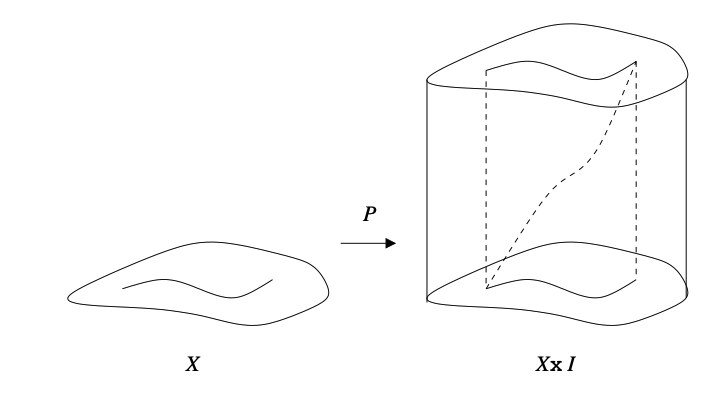
\includegraphics[scale = 0.25]{pictures/operadorprisma.png}
    \caption{Idea geomètrica de l'operador prisma}
    \label{fig:operadorprisma}
\end{figure}
Si l'espai topològic $X$ és arbitrari, no disposem de cap algorisme per realitzar aquesta subdivisió directament. La propera reducció consisteix en veure que és suficient, de fet, definir $P$ sobre els símplexs afins de $\Delta^q$.

Per poder realitzar aquesta reducció imposem una condició suplementària a l'operador prisma: que sigui natural en $X$. És a dir, volem definir operadors $P^X$ simultàniament sobre tots els espais topològics $X$ i de forma que, donada una aplicació contínua $h:Y\rightarrow X$ es tingui un diagrama commutatiu
\begin{equation}
    \notag
    \xymatrix{
    S_q(Y)\ar[r]^{P_q^Y}\ar[d]_{S_q(h)} & S_{q+1}(Y\times I)\ar[d]^{S_{q+1}(h\times \mathrm{id}_I)} \\
    S_q(X)\ar[r]^{P_q^X} & S_{q+1}(X\times I)
    }
\end{equation}
per a tot $q\geq 0$.

Sabem, a més, que és suficient definir $P_q^X$ sobre els generadors de $S_q(X)$.

Sigui $\sigma:\Delta^q\longrightarrow X$ un $q$-símplex singular. Per la naturalitat imposada a l'operador prisma, el diagrama
\begin{equation}
    \notag
    \xymatrix{
    S_q(Y)\ar[r]^{P_q^Y}\ar[d]_{S_q(\sigma)} & S_{q+1}(Y\times I)\ar[d]^{S_{q+1}(\sigma\times \mathrm{id}_I)} \\
    S_q(X)\ar[r]^{P_q^X} & S_{q+1}(X\times I)
    }
\end{equation}
ha d'ésser commutatiu. Observem que, si notem $\iota_q\in S_q(\Delta^q)$ el $q$-símplex singular corresponent a la identitat de $\Delta^q$, es té
\begin{equation}
    \notag
    S_q(\sigma)(\iota_q) = \sigma\circ\iota_q = \sigma\in S_q(X)
\end{equation}
i per tant, la commutativitat del diagrama anterior dóna la igualtat
\begin{equation}
    \notag
    P_q^X(\sigma) = S_{q+1}(\sigma\times\mathrm{id})P_q^{\Delta^q}(\iota_q)
\end{equation}
és a dir, la imatge de $\sigma$ per $P_q^X$, $P_q^X(\sigma)$, queda determinada pel valor de $P_q^{\Delta^q}(\iota_q)$.

En primer lloc observem que, prenent aquesta igualtat com a definició de $P_q^X$, la naturalitat és immediata: si $h:Y\rightarrow X$ és una aplicació contínua i $\sigma\in S_q(Y)$, es té
\begin{equation}
    \notag
    \begin{array}{ll}
        P_q^X(S_q(\sigma)) & = S_{q+1}((h\circ\sigma)\times \mathrm{id}_I)(\iota_q) \\
         & = S_{q+1}(h\times\mathrm{id}_I)S_{q+1}(\sigma\times \mathrm{id}_I)(\iota_q) \\
         &= S_{q+1}(h\times\mathrm{id}_I)P_q^Y(\sigma).
    \end{array}
\end{equation}
A més a més, la relació d'homotopia entre $S_\bullet(\lambda_0^X)$ i $S_\bullet(\lambda_1^X)$ es dedueix de la corresponent relació per $X = \Delta^q$ i $\sigma = \iota_q$:
\begin{equation}
    \notag
    (S_q(\lambda_1^{\Delta^q})-S_q(\lambda_0^{\Delta^q}))(\iota_q) = (\partial_{q+1}P_q^{\Delta^q}+P_{q-1}^{\Delta^q}\partial_q)(\iota_q),
\end{equation}
ja que aleshores es verificaran les igualtats
\begin{equation}
    \notag
    \begin{array}{ll}
        (S_q(\lambda_1^X)-S_q(\lambda_0^X))(\sigma) & = (S_q(\lambda_1^X)-S_q(\lambda_0^X))S_q(\sigma)(\iota_q) \\
         & = S_q(\sigma\times\mathrm{id})(S_q(\lambda_1^\Delta)-S_q(\lambda_0^\Delta))(\iota_q) \\
         & = S_q(\sigma\times\mathrm{id})(\partial_{q+1}P_q^\Delta(\iota_q)+P_{q-1}^\Delta\partial_q(\iota_q)) \\
         & = \partial_{q+1}S_{q+1}(\sigma\times\mathrm{id})(P_q^\Delta(\iota_q))+S_q(\sigma\times \mathrm{id})P_{q-1}^\Delta\partial_q(\iota_q)\\
         &= \partial_{q+1}P_q^X(\sigma)+P_{q-1}^X\partial_q(\sigma)
    \end{array}
\end{equation}

Per definir l'operador prisma sobre $\Delta^q$ aprofitarem la geometria afí dels símplexs estàndards. Considerarem $\Delta^q\subset\mathbb{R}^{q+1}$ amb vèrtexs $\{e_0,e_1,\ldots,e_q\}$, i sobre $\Delta^q\times I\subset \mathbb{R}^{q+1}\times I$ considerem els punts
\begin{equation}
    \notag
    \begin{array}{ll}
        a_0 = (e_0,0),\quad a_1 = (e_1,0),\quad\cdots,\quad a_q = (e_q,0)\\
        b_0 = (e_0,1),\quad b_1 = (e_1,1),\quad\cdots,\quad b_q = (e_q,1).
    \end{array}
\end{equation}
La figura \ref{fig:prismasobredelta2} mostra els punts $a_i,b_i$ en el cas $q = 2$.
\begin{figure}
    \centering
    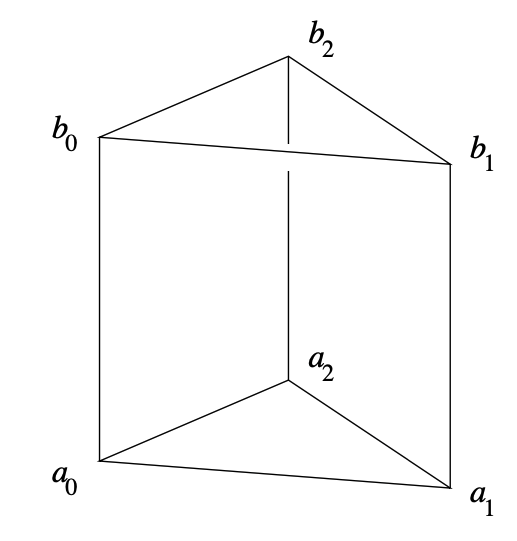
\includegraphics[scale = 0.25]{pictures/prismasobredelta2.png}
    \caption{Prisma sobre $\Delta^2$}
    \label{fig:prismasobredelta2}
\end{figure}

Els símplexs singulars afins de $\Delta^q$ i de $\Delta^q\times I$ estan determinats pels seus vèrtexs ordenats, pel que si $\sigma$ és un $q$-símplex singular afí el denotarem per $(\sigma(0),\ldots,\sigma(q))$. Així, per exemple, $\iota_q$ correspon al símplex $(e_0,\ldots,e_q)$. 

Ara es defineix l'operador prisma per 
\begin{equation}
    \notag
    P_q(e_0,e_1,\ldots,e_q) := \sum_{i=0}^q(-1)^{i}(a_0,a_1,\ldots,a_i,b_i,\ldots,b_q).
\end{equation}
Per exemple, per $q = 1$, tindrem $P_1(e_0,e_1) = (a_0,b_0,b_1)-(a_0,a_1,b_1)$, i per $q = 2$ tindrem
\begin{equation}
    \notag
    P_2(e_0,e_1,e_2) = (a_0,b_0,b_1,b_2)-(a_0,a_1,b_1,b_2)+(a_0,a_1,a_2,b_2).
\end{equation}

Provem ara que $P$ verifica la relació d'homotopia
\begin{equation}
    \notag
    (\partial_{q+1}P_q+P_{q-1}\partial_q)(\iota_q)=(S_q(\lambda_1)-S_q(\lambda_0))(\iota_q).   
\end{equation}
D'una banda tenim
\begin{equation}
    \notag
    \partial_{q+1}P_q(e_0,\ldots,e_q) = \partial_{q+1}\left(\sum_{i=0}^q(-1)^{i}(a_0,\ldots,a_i,b_i,\ldots,b_q)\right) = 
\end{equation}
\begin{equation}
    \notag
    = \sum_{i=0}^q(-1)^{i}\partial_{q+1}(a_0,\ldots,a_i,b_i,\ldots,b_q) = 
\end{equation}
\begin{equation}
    \notag
    = \sum_{i=0}^q(-1)^{i}\left(\sum_{0\leq j\leq i}(-1)^j(a_0,\ldots,\hat{a}_j,\ldots,a_i,b_i,\ldots,b_q)+\sum_{i\leq j\leq q}(-1)^{j+1}(a_0,\ldots,a_i,b_i,\ldots,\hat{b}_j,\ldots,b_q)\right)    
\end{equation}
Els termes $i = j$ apareixen en els dos sumatoris anteriors però amb signe canviat i per tant es cancel·len dos a dos, llevat de $(b_0,\ldots,b_q)$ i $(a_0,\ldots,a_q)$, pel que podem agrupar la suma anterior de la forma
\begin{equation}
    \notag
    (b_0,\ldots,b_q)+\sum_{0\leq j,i\leq q}(-1)^{i+j})a_0,\ldots,\hat{a}_j,\ldots,a_i,b_i,\ldots,b_q)+\sum_{0\leq i<j\leq q}(-1)^{i+j+1}(a_0,\ldots,a_i,b_i,\ldots,\hat{b}_j,\ldots,b_q)-(a_0,\ldots,a_q).
\end{equation}
D'altra banda, tenim
\begin{equation}
    \notag
    P_{q-1}\partial_q(e_0,\ldots,e_q) = P_{q-1}\left(\sum_{j=0}^q(-1)^j(e_0,\ldots,\hat{e}_j,\ldots,e_q)\right) = 
\end{equation}
\begin{equation}
    \notag
    = \sum_{j=0}^q(-1)^jP_{q-1}(e_0,\ldots,\hat{e}_j,\ldots,e_q) = 
\end{equation}
\begin{equation}
    \notag
    = \sum_{j=0}^q(-1)^j\left(\sum_{0\leq i<j}(-1)^{i}(a_0,\ldots,a_i,b_i,\ldots,\hat{b}_j,\ldots,b_q) + \sum_{j<i\leq q}(-1)^{i-1}(a_0,\ldots,\hat{a}_j,\ldots,a_i,b_i,\ldots,b_q)\right)    
\end{equation}
pel que, certament, es té
\begin{equation}
    \notag
    (\partial_{q+1}P_q+P_{q-1}\partial_q)(e_0,\ldots,e_q) = (b_0,\ldots,b_q)-(a_0,\ldots,a_q) = (S_q(\lambda_1)-S_q(\lambda_0))(e_0,\ldots,e_q),
\end{equation}
el que acaba, per fi, la demostració més llarga del mon.
\end{proof}

Com a conseqüència immediata d'aquest resultat trobem la invariància homotòpica de l'homologia singular dels espais topològics.

\begin{coro}
Siguin $X,Y$ espais topològics del mateix tipus d'homotopia. Llavors, els grups d'homologia singular de $X$ i $Y$ són isomorfs, és a dir, $H_\bullet(X)\cong H_\bullet(Y)$.
\end{coro}

\begin{ej}
\begin{enumerate}
    \item Sigui $X$ un espai topològic contràctil. Del càlcul de l'homologia singular d'un punt (que s'ha fet a l'apartat 1) i del corol·lari anterior, es deueix que 
    \begin{equation}
        \notag
        H_0(X)\cong\mathbb{Z},\qquad H_p(X)\cong 0,\;p\geq 1
    \end{equation}
    En particular, $\forall n$ $H_0(\mathbb{R}^n)\cong \mathbb{Z}\cong H_0(\Delta^n)$ i $H_p(\mathbb{R}^n)\cong 0\cong H_p(\Delta^n)$, per $p\geq 1$.
    
    Cal tenir en compte que hi ha espais topològics que tenen l'homologia d'un espai contràctil, però que no són contràctils.
    
    \item L'espai $\mathbb{R}^{n+1}\setminus\{0\}$ és del tipus d'homotopia de l'esfera $\mathbb{S}^n$ i, per tant, $H_p(\mathbb{R}^{n+1}\setminus\{0\})H_p(\mathbb{S}^n)$. Més endavant calcularem l'homologia de l'esfera i podrem acabar això.
\end{enumerate}
\end{ej}



Per acabar aquesta secció, veurem una aplicació particular d'aquest teorema relacionada amb els sespais contràctils. Primer, però, calen un parell de definicions.

\begin{defi}
[Homotopia de complexos de cadenes] Siguin $(M_\bullet,\partial_\bullet)$ i $(M_\bullet',\partial_\bullet')$ complexos de $R$-mòduls. Siguin $f,g:M_\bullet\rightarrow M_\bullet'$ morfismes de complexos de cadenes. Direm que $f$ i $g$ són homòtopes, i es denota $f\sim g$, si $\exists\{h_n\}_n$ tal que $h_p:M_p\rightarrow M_{p+1}'$, $\forall p\geq 1$ són morfismes de $R$-mòduls i
\begin{equation}
    \notag
    f_p-g_p = \partial_{p+1}'\circ h_p+h_{p-1}\circ\partial_p\qquad \forall p\geq 0
\end{equation}
\end{defi}


\begin{defi}[Complex de $R$-mòduls contràctil]
Sigui $(M_\bullet,\partial_\bullet)$ un complex de $R$-mòduls. Direm que és \textit{contràctil}\index{Contràctil} si $\mathrm{id}_{M_\bullet}\sim 0$, és a dir, si existeixen aplicacions $\{h_p:M_p\rightarrow M_{p-1}\}_p$ tals que $\mathrm{id}_p = \partial_{p+1}h_p + h_{p-1}\partial_p$, per tot $p\geq 0$. Si existeixen $\{h_p:M_p\rightarrow M_{p-1}\}_{p\geq n_0}$ tal que $\mathrm{id}_p = \partial_{p+1}h_p+h_{p-1}\partial_p$ es verifica $\forall p\geq n_0$, es diu que $(M_\bullet,\partial_\bullet)$ és contràctil en grau més gran que $n_0$.
\end{defi}

\begin{lema}
Si $(M_\bullet,\partial_\bullet)$ és contràctil en grau més gran que $n_0$, aleshores $H_p(M_\bullet) = 0$ per tot $p>n_0$. En particular, si $(M_\bullet,\partial_\bullet)$ és contràctil, aleshores $H_p(M_\bullet) = 0$ per tot $p\geq 0$).
\end{lema}
\begin{proof}
Es deixa com a exercici.
\end{proof}

\begin{prop}
A tall d'exemple, fem aquesta proposició que és un exemple molt general. Sigui $X\subset\mathbb{R}^N$ fitat i convex. Aleshores, $S_\bullet(X,R)$ és contràctil en grau més gran que 0. Per tant, $H_p(X) = 0$ si $p>0$.
\end{prop}
\begin{proof}
Es deixa com a exercici.
\end{proof}



\section{El teorema de les cadenes petites}

En aquest apartat provarem el teorema de les cadenes petites, resultat fonamental de l'homologia singular que ens permetrà provar més endavant el teorema de Mayer-Vietoris i d'escissió. El terme \textit{cadena petita} fa referència al tamany d'una cadena respecte d'un recobriment, com ara precisem.

\begin{defi}
Sigui $X$ un espai topològic, sigui $\mathcal{U} = \{U_i\}_{i\in I}$ un recobriment de $X$. Una cadena singular $c\in S_p(X)$ és $\mathcal{U}$-\textit{petita} si prenent $c = \sum_{j=1}^n\lambda_j\sigma_j$, $\sigma_j:\Delta^p\rightarrow X$, llavors $\forall j\in\{1,\ldots,n\}$ $\exists i\in I$ tq $\sigma_j(\Delta^p)\subset U_i$. És a dir, si tota la cadena cau a dins d'un dels oberts.
\end{defi}


\begin{ej}
Sigui $X = \mathbb{S}^n$, $U_1 = \mathbb{S}^n\cap\{\mathbf{x}\in\mathbb{R}^{n+1}\;:\;x_n\geq 0$ i $U_2 = \mathbb{S}^n\cap\{\mathbf{x}\in\mathbb{R}^{n+1}\;:\;x_n\leq 0\}$, és a dir, el recobriment per oberts que són l'hemisferi nord, $E_+^n$ i sud, $E_-^n$. Llavors, una cadena que sigui per exemple recórrer un paral·lel (que no sigui l'Equador) és una cadena $\mathcal{U}$-petita. En canvi, un meridià no ho és.
\end{ej}


Podem considerar el complex $(S_\bullet(\mathcal{U}),\partial_\bullet)$ que és un complex de cadenes
\begin{equation}
    \notag
    S_\bullet(\mathcal{U})\hookrightarrow S_\bullet(X)
\end{equation}
Per tant tenim $\forall p\geq 0$,
\begin{equation}
    \notag
    H_p(S(\mathcal{U}))\longrightarrow H_p(X)
\end{equation}
\begin{ej}
$X = \mathbb{S}^1$ i $\tau$ la topologia estàndard. Prenem $\mathcal{U} = \{\{x\}\;:\;x\in\mathbb{S}^1\}$. Llavors, $H_0(S_\bullet(\mathcal{U}))$ és molt més gran.
\end{ej}



\begin{ter}
[Cadenes petites]\index{Teorema de les cadenes petites} Si $\mathcal{U} = \{U_i\}_{i\in I}$ és un recobriment de $X$ tal que $X = \bigcup_{i\in I} \overset{\circ}{U_i}$, aleshores els morfismes
\begin{equation}
    \notag
    H_p(S_\bullet(\mathcal{U}))\longrightarrow H_p(X)
\end{equation}
són isomorfismes $\forall p\geq 0$.
\end{ter}

La idea de la demostració del teorema de les cadenes petites consisteix en provar que, per un procés de subdivisió baricèntrica anàleg al desenvolupat en el capítol 1, tota cadena singular de $X$ és homòloga a una cadena $\mathcal{U}$-petita. Per exemple, en el cas del meridià de $\mathbb{S}^n$ de l'exemple del rpincipi d'aquest paràgraf, podem subdividir-lo com una cadena formada per la suma de dos arcs, cadascun d'ells corresponent al tall amb els semiespais de $\mathbb{R}^{n+1}$ definits per $x_{n+1}\geq 0$ i $x_{n+1}\leq 0$, que és una cadena $\{E_+^n,E_-^n\}$-petita, on $E_+^n$ representa l'hemisferi nord de $\mathbb{S}^n$ i $E_-^n$ l'hemisferi sud.

Per a dur a terme aquesta idea, hem d'adaptar prèviament els conceptes i resultats de subdivisió baricèntrica del capítol 1 a l'homologia singular.

\begin{enumerate}
    \item \textit{Con d'un símplex singular afí.}\index{Con d'un símplex singular afí}
    
    Sigui $\sigma:\Delta^p\rightarrow\mathbb{R}^n$ un $p$-símplex singular afí, $\sigma = (a_0,a_1,\ldots,a_p)$, $a_i = \sigma(e_i)$. Si $b$ és un punt de $\mathbb{R}^n$, el \textit{con de vèrtex $b$ sobre $\sigma$} es defineix com el $(p+1)$-símplex singular afí determinat per
    \begin{equation}
        \notag
        b*\sigma:=(b,a_0,a_1,\ldots,a_p).
    \end{equation}
    
    Si $c = \sum_{i=1}^r\lambda_i\sigma_i$, $\lambda_i\in\mathbb{Z}$, és una $p$-cadena singular en la que els símplexs $\sigma_i$ són afins, definim
    \begin{equation}
        \notag
        b*c:=\sum_{i=0}^p\lambda_i(b*\sigma_i).
    \end{equation}
    
    \begin{lema}
    Es verifica
    \begin{enumerate}
        \item $\partial(b*c) = c-\left(\sum_{i=0}^p\lambda_i\right)b$, si $c = \sum_{i=0}^p\lambda_i\sigma_i$ és $0$-dimensional,
        \item $\partial(b*c) = c-b*\partial c$, si $c$ és una cadena $p$-dimensional, $p>0$.
    \end{enumerate}
    \end{lema}
    \begin{proof}
    Si $c$ és una cadena $0$-dimensional, $c = \sum_{i=0}^p\lambda_i(a_i)$, així
    \begin{equation}
        \notag
        \begin{array}{ll}
            \partial\left(b*\sum_{i=0}^p\lambda_i\sigma_i\right) & = \partial\left(\sum_{i=0}^p\lambda_ib*\sigma_i\right) = \sum_{i=0}^p\partial(b*\sigma_i) = \\
            &= \sum_{i=0}^p\lambda_i\partial(b,a_i) = \sum_{i=0}^p\lambda_i((a_i)-(b)) = \\
            &= c-\left(\sum_{i=0}^p\lambda_i\right)b.
        \end{array}
    \end{equation}
    Considerem ara el cas $p$-dimensional, amb $p>0$. Com ambdues parts de la igualtat són lineals en $c$, és suficient demostrar-la per als $p$-símplexs. Si $\sigma = (a_0,\ldots,a_p)$, es té
    \begin{equation}
        \notag
        \begin{array}{ll}
            \partial(b*\sigma) & = \partial(b,a_0,\ldots,a_p) =  \\
             & = (a_0,a_1,\ldots,a_p)-\sum_{i=0}^p(-1)^{i}(b,a_0,\ldots,\hat{a}_i,\ldots,a_p) = \\
             & = \sigma-b*\partial\sigma.
        \end{array}
    \end{equation}
    \end{proof}
    
    \item \textit{Operador de subdivisió baricèntrica}\index{Operador de subdivisió baricèntrica}.
    
    La subdivisió baricèntrica d'un símplex afí introduïda al capítol 1 permet escriure un tal símplex com una cadena formada per símplexs de talla tant petita com es vulgui. El resultat següent trasllada aquesta construcció a l'homologia singular.
    
    \begin{prop}
    [Divisió baricèntrica]\label{prop:divisiobaricentrica} Per a tot espai topològic $X$, existeix un morfisme de complexos
    \begin{equation}
    \notag
    \mathrm{sd}_\bullet^X:S_\bullet(X)\rightarrow S_\bullet(X)
    \end{equation}
    i morfismes
    \begin{equation}
    \notag
    h_p^X:S_p(X)\rightarrow S_{p+1}(X)\quad\forall p\geq 0\quad (h_{-1}^X = 0)
    \end{equation}
    tals que
    \begin{enumerate}[(a)]
        \item $\mathrm{sd}_*^X$ i $h_p^X$ són functorials, si $f:X\rightarrow Y$ és contínua
        \begin{equation}
        \notag
        \xymatrix{
        S_\bullet(X)\ar[r]^{\mathrm{sd}_\bullet^X}\ar[d]_{f_\bullet} & S_\bullet(X)\ar[d]^{f_\bullet} \\
        S_\bullet(Y)\ar[r]_{\mathrm{sd}_\bullet^Y} & S_\bullet(Y)
        }
        \end{equation}
        \begin{equation}
        \notag
        \xymatrix{
        S_p(X)\ar[r]^{h_p^X}\ar[d]_{f_p} & S_{p+1}(X)\ar[d]^{f_{p+1}} \\
        S_p(Y)\ar[r]_{h_p^Y} & S_{p+1}(Y)
        }
        \end{equation}
        \item $\{h_p^X\}_p$ és una homotopia entre $\mathrm{sd}_\bullet^X$ i $\mathrm{id}_{S_\bullet(X)}$.
        \item Si $\mathcal{U} = \{U_i\}{i\in I}$ és un recobriment de $X$ tal que $X = \bigcup_{i\in I} \overset{\circ}{U_i}$ i $z_p\in S_p(X)$, existeix $n\geq 0$ tal que $(\mathrm{sd}_p^X)^n(z_p)\in S_p(\mathcal{U})$.
    \end{enumerate}
    \end{prop}
    \begin{proof}
    Començarem definint l'operador $sd_p^X$, $p\geq 0$, i comprovarem que és un morfisme de complexos, inductivament sobre $p$. Com en la demostració del teorema d'invariància homotòpica (\ref{ter:invarianciahomotopica}), podem usar la naturalitat de $sd_p^X$ i assegurar que és suficient definir
    \begin{equation}
        \notag
        \begin{array}{rl}
            sd_p^\Delta: S_p(\Delta^p)& \longrightarrow S_p(\Delta^p) \\
            \iota_p & \longmapsto sd_p(\iota_p)
        \end{array}
    \end{equation}
    per tot $p\geq 0$. En efecte, si $\sigma$ és un $p$-símplex singular de $X$, el diagrama commutatiu
    \begin{equation}
        \notag
        \xymatrix{
        S_\bullet(\Delta^p)\ar[r]^{sd_\bullet^{\Delta^p}}\ar[d]_{S_\bullet(\sigma)} & S_\bullet(\Delta^p)\ar[d]^{S_\bullet(\sigma)} \\
        S_\bullet(Y)\ar[r]_{sd_\bullet^Y} & S_\bullet(X)
        }
    \end{equation}
    obliga aleshores a definir
    \begin{equation}
        \notag
        sd_p^X(\sigma):= S_p(\sigma_\bullet)(sd_p^{\Delta^p}(\iota_p)),
    \end{equation}
    on $\iota_p$ és el $p$-símplexs singular identitat $\iota_p:\Delta^p\rightarrow\Delta^p$.
    
    Sigui $b_p$ el baricentre de $\iota_p$, és a dir,
    \begin{equation}
        \notag
        b_p:=\frac{1}{p+1}\sum_{i=0}^p e_i
    \end{equation}
    Es defineix $sd_p^{\Delta^p}(\iota_p)$ inductivament segons
    \begin{equation}
        \notag
        sd_p^{\Delta^p}(\iota_p) := \left\{
        \begin{array}{ll}
            \iota_p, & \text{si $p = 0$}\\
            b_p*sd_{p-1}^{\Delta^{p-1}}(\partial\iota_p) & \text{si $p>0$},    
        \end{array}
        \right.
    \end{equation}
    que és una altra forma d'expressar la subdivisió baricèntrica del capítol 1 (que no vam fer...). Per exemple, per $p = 1$ trobem
    \begin{equation}
        \notag
        sd_1(\iota_1) = b_1*sd_0[(e_1)-(e_0)] = b_1*[(e_1)-(e_0)] = b_1*(e_1)-b_1*(e_0) = (b_1,e_1)-(b_0,e_0).
    \end{equation}
    
    Provem per inducció sobre $p$ que es verifica $sd_{p-1}^X\partial_p\sigma = \partial_psd_p^X\sigma$, per a tot $p$-símplex $\sigma$ d'un espai topològic qualsevol $X$. Per $p = 0$ el resultat és trivial, ja que $\partial_0 = 0$. Suposem per hipòtesi d'inducció que hem provat $sd_{q-1}^X\partial_q\sigma = \partial_qsd_q^X\sigma$, per tot $q$-símplex $\sigma$ d'un espai topològic qualsevol $X$, si $q<p$. Comencem provant que $sd_{p-1}\partial_p\iota_p = \partial_psd_p\iota_p$. Es té
    \begin{equation}
        \notag
        \begin{array}{lll}
            \partial_psd_p\iota_p &= \partial_p(b_p*sd_{p-1}\partial_p\iota_p) & \\
            & = sd_{p-1}\partial_p\iota_p-b_p*\partial_{p-1}sd_{p-1}\partial_p\iota_p & \text{pel lema anterior} \\
            & = sd_{p-1}\partial_p\iota_p-b_p*sd_{p-2}\partial_{p-1}\partial_p\sigma_p, & \text{per hipòtesi d'inducció}\\
            & = sd_{p-1}\partial_p\iota_p.
        \end{array}
    \end{equation}
    
    Com hem definit $sd_p^X$ per la igualtat $sd_p^X(\sigma) = S_p(\sigma)(sd_p^{\Delta^p}(\iota_p))$, observem que si $\sigma$ és un símplex afí, $sd_p^{\Delta^p}(\sigma)$ també és afí, i es verifica
    \begin{equation}
        \notag
        \begin{array}{ll}
            sd_{p-1}^X(\partial_p\sigma) & = sd_{p-1}^X(\partial_pS_p(\sigma)(\iota_p)) = sd_{p-1}^XS_{p-1}(\sigma)(\partial_p\iota_p)\\
            &= S_{p-1}(\sigma)sd_{p-1}^{\Delta^p}(\partial_p\iota_p) = S_{p-1}(\sigma)\partial_psd_p^{\Delta^p}(\iota_p)\\
            & = \partial_pS_p(\sigma)sd_p^{\Delta^p}(\iota_p) = \partial_psd_p^X(\sigma).
        \end{array}
    \end{equation}
    
    Respecte els morfismes $T_p^X$, una vegada més per la naturalitat imposada als operadors $T_p^X$, $p\geq 0$, i inducció, és suficient definir $T_p^{\Delta^p}(\iota_p)$, $\iota_p\in S_p(\Delta^p)$, tal que
    \begin{equation}
        \notag
        T_{p-1}\partial_p(\iota_p)+\partial_{p+1}T_p(\iota_p) = \mathrm{id}_p(\iota_p)-sd_p(\iota_p),
    \end{equation}
    on, per simplificar la notació, he escrit $T_p$ en lloc de $T_p^{\Delta^p}$. No segueixo perquè ja no puc més amb aquesta demostració hiper llarga. No trobo el sentit a la meva existència després de fer aquestes demostracions sense final de no sé quin teorema que ni entenc.
    
    Per demostrar l'apartat (c) utilitzarem les següents coses:
    \begin{defi}
    Sigui $X$ espai mètric i $A\subset X$. Definim el diàmetre de $A$ com
    \begin{equation}
    \notag
    \mathrm{diam}(A) = \sup_{x,y\in A}\{d(x,y)\}
    \end{equation}
    \end{defi}
    \begin{lema}
    [Nombre de Lebesgue]\label{lema:nombredelebesgue} Si $X$ és un espai mètric compacte i $\mathcal{U}$ un recobriment obert de $X$, aleshores existeix $\lambda>0$ (el nombre de Lebesgue) tal que per a tot subconjunt $A\subset X$ tal que $\mathrm{diam}(A)<\lambda$, $\exists U\in \mathcal{U}$ tal  que $A\subset U$.
    \end{lema}
    \begin{defi}
    Direm que $\tau:\Delta^p\rightarrow \Delta^p$ és afí si 
    \begin{equation}
    \notag
    \tau\left(\sum_i t_ie_i\right) = \sum_i t_i\tau(e_i)
    \end{equation}
    \end{defi}
    \begin{lema}
    Si $\tau:\Delta^p\rightarrow \Delta^p$ afí, tot símplex $\eta$ de $\mathrm{sd}_p^{\Delta^p}(\tau)$ és afí i verifica
    \begin{equation}
    \notag
    \mathrm{diam}(\eta) \leq \frac{p}{p+1}\mathrm{diam}(\tau)
    \end{equation}
    \end{lema}
    \begin{proof}
    Siguin $x_0,\ldots,x_p$ els vèrtexs de $\tau$. Per convexitat, tenim
    \begin{equation}
    \notag
    \mathrm{diam}(\tau) = \max\{\|x_i-y_j\|\}
    \end{equation}
    Llavors, tots els símplexs de la subdivisió baricèntrica contenen algun $x_i$ i el baricentre $b_p = \frac{1}{p+1}\sum_i = x_i$. No és difícil veure (es deixa com a exercici) que $\mathrm{diam}(\eta) = \|b-x_{i_0}\| = \frac{1}{p+1}\left\|\sum_{i=0}^px_i-(p+1)x_{i_0}\right\|$ i a més, per la desigualtat triangular:
    \begin{equation}
    \notag
    \mathrm{diam}(\eta) = \|b-x_{i_0}\| = \frac{1}{p+1}\left\|\sum_{i=0}^px_i-(p+1)x_{i_0}\right\|\leq \frac{1}{p+1}\sum_{i=0}^p\|x_i-x_j\|
    \end{equation}
    que té $p$ termes. Ara bé, cadascun d'aquests termes és més petit o igual al diàmetre, i.e.
    \begin{equation}
    \notag
    \mathrm{diam}(\eta)\leq \frac{p}{p+1}\mathrm{diam}(\tau)
    \end{equation}
    \end{proof}
    \begin{coro}
    Tot símplex $\eta$ de $\mathrm{sd}^{\Delta^p}(\mathrm{id}_p)$ és afí i $\mathrm{diam}(\eta)\leq\frac{p}{p+1}\mathrm{diam}(\Delta^p)$.
    \end{coro}
    Ara ja podem fer la demostració de l'apartat (c) del teorema de divisió baricèntrica.


    Podem suposar que $z = \sigma:\Delta^p\rightarrow X$. Com $\{\overset{\circ}{U_i}\}_{i\in I}$ és un recobriment de $X$, $\{\sigma^{-1}(\overset{\circ}{U_i})\}_{i\in I}$ és recobriment de $\Delta^p$. Com $\Delta^p$ és espai mètric compacte, $\exists\lambda>0$ nombre de Lebesgue del recobriment. Sigui $n$ suficientment gran tal que $\left(\frac{p}{p+1}\right)^n<\lambda$. Aleshores $\mathrm{diam}(\mathrm{sd}^n(\mathrm{id}_p))<\lambda$. Tots els símplexs de $\mathrm{sd}^n(\mathrm{id}_p)$ són a dins d'algun $\sigma^{-1}(\overset{\circ}{U_i})$. Aplicar $\sigma$ i ja està.
    \end{proof}
    
    \begin{coro}
    El morfisme de complexos de cadenes $\mathrm{sd}_\bullet^X:S_\bullet(X)\rightarrow X_\bullet(X)$ indueix
    \begin{equation}
    \notag
    H_p(X)\rightarrow H_p(X)\quad\forall p\geq 0
    \end{equation}
    i pel teorema d'abans això és l'aplicació identitat.
    \end{coro}


    \begin{nota}
    $\mathrm{sd}_\bullet\sim \mathrm{id}$ on la relació és d'homotopia. D'aquí, $(\mathrm{sd}_\bullet)^n = \mathrm{sd}_\bullet\circ(\mathrm{sd}_\bullet)^{n-1}\sim \mathrm{id}$. És a dir, si posem $s = \mathrm{sd}_\bullet$ i $1 = \mathrm{id}_{S_\bullet(X)}$, tenim
    \begin{equation}
    \notag
    (s^n-1) = (\underbrace{s^{n-1}+s^{n-2}+\cdots+1}_g)(s-1=
    \end{equation}
    i així això és igual a 
    \begin{equation}
    \notag
    g(s-1) = g(\partial h+h\partial) = (gh)\partial + \partial(gh)
    \end{equation}
    \end{nota}
    
    \item \begin{proof}[Demostració del teorema de les cadenes petites]
    La inclusió $S_\bullet(\mathcal{U})\hookrightarrow S_\bullet(X)$ indueix per pas al quocient una successió exacta de complexos
    \begin{equation}
        \notag
        0\rightarrow S_\bullet(\mathcal{U})\rightarrow S_\bullet(X)\rightarrow S_\bullet(X)/S_\bullet(\mathcal{U})\rightarrow 0
    \end{equation}
    que alhora, indueix una successió exacta llarga d'homologia
    \begin{equation}
        \notag
        \cdots\rightarrow H_{p+1}\left(\frac{S_\bullet(X)}{S_\bullet(\mathcal{U})}\right)\rightarrow H_p(S_\bullet(\mathcal{U})\rightarrow H_p(X)\rightarrow H_p\left(\frac{S_\bullet(X)}{S_\bullet(\mathcal{U})}\right)\rightarrow\cdots
    \end{equation}
    pel que és suficient provar que $H_p(S_\bullet(X)/S_\bullet(\mathcal{U})) = 0$ per a tot $p\geq 0$.
    
    Sigui $[z]\in H_p(S_\bullet(X)/S_\bullet(\mathcal{U}))$ una classe d'homologia representada per $z\in S_p(X)$. Observem, en primer lloc, que $z$ i $sd(z)$ són cicles homòlegs del complex $S_\bullet(X)/S_\bullet(\mathcal{U})$. En efecte, com $z$ és un cicle, verifica $\partial(z) \in S_{p-1}(\mathcal{U})$, és a dir, la cadena $\partial(z)$ és una cadena $\mathcal{U}$-petita. Aplicant a $z$ la igualtat
    \begin{equation}
        \notag
        \mathrm{id}_p-sd_p = \partial_{p+1}T_p+T_{p-1}\partial_p
    \end{equation}
    obtinguda en el paràgraf anterior, trobem que $z-sd(z) = \partial T(z)+T\partial(z)$, com elements de $S_\bullet(X)$. Ara, com que $T$ és una homotopia natural, la inclusió de $U_i$ en $X$ dona lloc a un diagrama commutatiu
    \begin{equation}
        \notag
        \xymatrix{
        S_p(U_i)\ar[r]^{T_p^{U_i}}\ar[d] & S_{p+1}(U_i)\ar[d]\\
        S_p(X)\ar[r]^{T^X_p}& S_{p+1}(X)
        }
    \end{equation}
    el que mostra que $T\partial (z)$ també és $\mathcal{U}$-petita. Per tant, $z-sd(z) = \partial T(z)$ a $S_\bullet(X)/S_\bullet(\mathcal{U})$ i passant a homologies tindrem $[z]-[sd(z)] = 0$ en $H_p(S_\bullet(X)/S_\bullet(\mathcal{U}))$. En definitiva,
    \begin{equation}
        \notag
        [z] = [sd(z)]\in H_p(S_\bullet(X)/S_\bullet(\mathcal{U})).
    \end{equation}
    Així, per inducció es verifica
    \begin{equation}
        \notag
        [z] = [sd(z)] = [sd^2(z)] = \cdots = [sd^n(z)]\quad \text{a}\quad H_p(S_\bullet(X)/S_\bullet(\mathcal{U}))
    \end{equation}
    Però, pel teorema (\ref{prop:divisiobaricentrica}) existeix un $n$ tal que $sd^n(z)$ és $\mathcal{U}$-petita, i per tant és igual a zero en $H_p(S_\bullet(X)/S_\bullet(\mathcal{U}))$. 
    \end{proof}
\end{enumerate}

En les condicions del teorema de les cadenes petites, el morfisme de complexos $S_\bullet(\mathcal{U})\rightarrow S_\bullet(X)$ no solament indueix un isomorfisme en homologia sinó que, de fet, és una equivalència homotòpica de complexos. La versió que hem donat serà suficient per les necessitats d'aquests apunts, però la versió general del resultat consisteix a provar això mateix.




\section{La successió exacta de Mayer-Vietoris}
El teorema de Mayer-Vietoris que enunciem a continuació és el resultat anàleg, en homologia singular, al corresponent teorema de l'homologia simplicial. Aquest resultat, juntament amb la invariància homotòpica de l'homologia singular, ens permetrà calcular els grups d'homologia de les esferes, i donar les primeres aplicacions geomètriques de l'homologia singular.

Sigui $X$ un espai topològic i $U$ i $V$ dos subconjunts de $X$ tals que $X = U^\circ\cup V^\circ$. Sigui $\pi$ el morfisme de complexos
\begin{equation}
    \notag
    \begin{array}{rl}
        \pi:S_\bullet(U)\oplus S_\bullet(V) & \longrightarrow S_\bullet(X) \\
        (c_1,c_2) & \longmapsto c_1-c_2
    \end{array}
\end{equation}
i notem per $\iota$ el morfisme induit per la inclusió
\begin{equation}
    \notag
    \begin{array}{rl}
        \iota:S_\bullet(U\cap V) & \longrightarrow S_\bullet(U)\oplus S_\bullet(V) \\
        c & \longmapsto (c,c)
    \end{array}
\end{equation}


\begin{ter}
Amb les notacions anteriors, existeix un morfisme $\partial_{U,V}:H_p(X)\rightarrow H_{p-1}(U\cap V)$, per a tot $p\geq 0$, tal que la successió
\begin{equation}
    \notag
    \cdots \rightarrow H_p(U\cap V)\overset{\iota_\bullet}{\longrightarrow}H_p(U)\oplus H_p(V)\overset{\pi_\bullet}{\longrightarrow} H_p(X)\overset{\partial_{U,V}}{\longrightarrow}H_{p-1}(U\cap V)\rightarrow\cdots
\end{equation}
és exacta.
\end{ter}

Aquesta successió exacta és natural en $U,V$, i s'anomena la \textit{successió exacta de Mayer-Vietoris}\index{Successió exacta de Mayer-Vietoris} del recobriment $\{U,V\}$.

\begin{proof}
Sigui $\mathcal{U}$ el recobriment de $X$ format per $U$ i $V$. La imatge del morfisme
\begin{equation}
    \notag
    \begin{array}{rl}
        \pi:S_\bullet(U)\oplus S_\bullet(V) & \longrightarrow S_\bullet(X) \\
        (c_1,c_2) & \longmapsto c_1-c_2
    \end{array}
\end{equation}
és exactament $S_\bullet(\mathcal{U})$, mentre que el seu nucli està format per les parelles $(c_1,c_2)\in S_\bullet(U)\oplus S_\bullet(V)$ tals que $c_1 = c_2$, i per tant, $c_1 = c_2\in S_\bullet(U\cap V)$. És a dir, es té la successió exacta de complexos
\begin{equation}
    \notag
    0\longrightarrow S_\bullet(U\cap V)\longrightarrow S_\bullet(U)\oplus S_\bullet(V)\longrightarrow S_\bullet(\mathcal{U})\longrightarrow 0
\end{equation}
Prenent la successió exacta llarga d'homologia tenim
\begin{equation}
    \notag
    \cdots \rightarrow H_p(U\cap V)\overset{\iota_\bullet}{\longrightarrow}H_p(U)\oplus H_p(V)\overset{\pi_\bullet'}{\longrightarrow} H_p(X)\overset{\partial_{U,V}'}{\longrightarrow}H_{p-1}(U\cap V)\rightarrow\cdots
\end{equation}
Però pel teorema de les cadenes petites aplicat al recobriment $\mathcal{U}$, es té isomorfisme $j_\bullet:H_\bullet(S_\bullet(\mathcal{U}))\overset{\sim}{\longrightarrow}H_\bullet(X)$, induit per la inclusió del complex $S_\bullet(\mathcal{U})$ en el complex $S_\bullet(X)$. Així, $j_\bullet\pi_\bullet' = \pi_\bullet$, i per tant podem substituir $H_\bullet(S_\bullet(\mathcal{U}))$ per $H_\bullet(X)$ en la successió exacta anterior, $\pi_\bullet'$ per $\pi_\bullet$, i finalment definir $\partial_{U,V} = \partial_{U,V}'(j_\bullet^{-1})$, amb el que es verifica l'enunciat del teorema.
\end{proof}

Observem que la successió de Mayer-Vietoris depèn de l'ordre del recobriment $\{U,V\}$ de $X$ ja que aquest ordre determina el morfisme
\begin{equation}
    \notag
    \pi_\bullet:S_\bullet(U)\oplus S_\bullet(V)\longrightarrow S_\bullet(\mathcal{U})\longrightarrow 0
\end{equation}
Si invertim l'ordre, aleshores el morfisme resultant
\begin{equation}
    \notag
    -\pi:S_\bullet(V)\oplus S_\bullet(U)\longrightarrow S_\bullet(X)
\end{equation}
és l'oposat al considerat pel recobriment $\mathcal{U}$, així és immediat completar el teorema de Mayer-Vietoris de la següent forma
\begin{coro}
Si en el teorema anterior invertim l'ordre del recobriment, aleshores $\partial_{V,U} = -\partial_{U,V}$. Així, la successió exacta de Mayer-Vietoris que li correspon és la mateixa però invertida i canviant $\pi_\bullet$ per $-\pi_\bullet$.
\end{coro}

Veiem ara una aplicació d'aquest teorema en el càlcul de l'homologia de les esferes.

\section{Càlcul d'homologies singulars}


Com a aplicació de la successió exacta de Mayer-Vietoris calcularem l'homologia singular de les esferes.

Considerem en primer lloc la circumferència $\mathbb{S}^1$. Siguin $A,B$ dos punts diferents de $\mathbb{S}^1$, i descomponem $\mathbb{S}^1$ de la forma
\begin{equation}
    \notag
    \mathbb{S}^1 = (\mathbb{S}^1\setminus A)\cup(\mathbb{S}^1\setminus B).
\end{equation}
Aleshores, si prenem $U = \mathbb{S}^1\setminus A\simeq\mathbb{R}$ i $V = \mathbb{S}^1\setminus B\simeq \mathbb{R}$ tindrem $U\cap V\simeq \mathbb{R}\sqcup\mathbb{R}$. Tenim doncs,
\begin{itemize}
    \item $H_0(U)\cong\mathbb{Z}$. Això és perquè és contràctil i ja vam veure quin era l'homologia singular de l'espai topològic amb un sol punt. Utilitzant això i el teorema d'invariància homotòpica s'obté aquesta homologia. Un generador és $[p]$, per a $p\in U$ i aleshores $H_0(U)\cong\mathbb{Z}$, $\forall p\in U$. El mateix passa amb $H_0(V)\cong \mathbb{Z}[q]$, per qualsevol $q\in V$. Notem que podria donar-se que $p$ i $q$ fossin els mateixos, però prendrem $p\not=q$. Ara bé, si considerem el símplex $\sigma:\Delta^1\rightarrow \Delta^1$ tal que $\sigma(p)=q$, aleshores $\partial\sigma = [p]-[q] = 0$ ja que en $H_0(U)$ o en $H_0(V)$, $[p] = [q]$. Ara bé, compte! Perquè si haguéssim pres $p = A$ o $q = B$ tot això és mentida! Per tant hem de prendre $p$ i $q$ de $U$ i de $V$ respectivament, que ja és el que hem fet. Això implica que està ben generat.
    
    \item Calculem ara $H_0(U\cap V)$. És clar que l'homologia simplicial serà
    \begin{equation}
        \notag
        H_0(U\cap V) \cong\mathbb{Z}[p]\oplus\mathbb{Z}[q]
    \end{equation}
\end{itemize}   

Busquem ara l'aplicació $f:H_0(U\cap V)\rightarrow H_0(U)\oplus H_0(V)$. Notem que si prenem $[p],[q]\in H_0(U\cap V)$ amb $p\in U\setminus V$ i $q\in V\setminus U$ com abans, aleshores $[p]\not=[q]$ en $H_0(U\cap V)$, però $[p] = [q]$ en $H_0(U)\oplus H_0(V)$. Per tant, podem prendre l'aplicació que envia $[p]\mapsto([p],[p])$ i $[q]\mapsto([q],[q])=([p],[p])$. Per tant, tenim la successió
\begin{equation}
    \notag
    \cdots \rightarrow H_1(\mathbb{S}^1)\overset{\partial}{\longrightarrow} H_0(U\cap V)\overset{f}{\longrightarrow} H_0(U)\oplus H_0(V)\longrightarrow H_0(\mathbb{S}^1)
\end{equation}
on $\ker f = \langle [p]-[q]\rangle$ pel que hem dit abans. 

El morfisme de connexió és ara
\begin{equation}
    \notag
    \xymatrix{
    0 \ar[r] & S_1(U\cap V)\ar[r]\ar[d] & S_1(U)\oplus S_1(V)\ar[r]\ar[d] & S_1(\{U,V\})\ar[d]\\
    0 \ar[r] & S_0(U\cap V)\ar[r] & S_0(U)\oplus S_0(V)\ar[r] & S_0(\{U,V\})
    }
\end{equation}
Llavors, si aconseguim calcular $S_1(\{U,V\})$ (generadors), aleshores sabem que $H_1(\mathbb{S}^1)\cong H_1(S_1(\mathbb{S}^1))$ i com que $U$ i $V$ són un recobriment de $\mathbb{S}^1$, $\mathbb{S}^1\simeq \{U,V\}$. 

Llavors, si prenem els camins
\begin{equation}
    \notag
    \begin{array}{rl}
        \alpha:\left[0,1\right] & \longrightarrow U \\
        t & e^{2\pi i\left(1-\frac{t}{2}\right)}
    \end{array}\qquad
    \begin{array}{rl}
        \beta:\left[0,1\right] & \longrightarrow V \\
        t & \longmapsto e^{2\pi i\left(\frac{1-t}{2}\right)}
    \end{array}
\end{equation}
tenim que $\alpha+\beta$ és un generador de $S_1(\{U,V\})$. Anem a provar això. Primer notem que, si situem $\mathbb{S}^1$ com la circumferència centrada en $(0,0)$ i radi 1, de manera que els punts que hem extret siguin el pol nord i sud, i situem $p = (1,0)$ i $q = (-1,0)$ per a que tot sigui més visual, aquests camins no són més que recórrer l'hemisferi sud de $p$ a $q$ (en el cas de $\alpha$) i el nord de $p$ a $q$ també (en el cas de $\beta$). Ara observem que $\partial(\alpha+\beta) = 0$ trivialment, ja que $\partial\alpha = [q]-[p]$ i $\partial\beta = [p]-[q]$. El que s'ha de fer és pensar en $\alpha$ i $\beta$ com a 1-símplexs singulars, ja que $[0,1] = \Delta^1$ i $U$ i $V$ són els espais topològics de sortida. Aleshores, podem veure què fa el morfisme de connexió amb $\alpha$ i $\beta$:
\begin{equation}
    \notag
    \begin{array}{rl}
        S_1(U)\oplus S_1(V) & \longrightarrow S_0(U)\oplus S_0(V) \\
        (\alpha,-\beta) & \longmapsto (\left[q\right]-\left[p\right], \left[q\right]-\left[p\right])
    \end{array}
\end{equation}

O sigui, mirant el morfisme de connexió, el que hem de fer és, sabent els generadors de $S_0(U\cap V)$, anar definint morfismes per poder saber a on van a parar aquests generadors quan arribem a $S_1(\{U,V\})$. Llavors, hem començat ara dient que $S_0(U)\oplus S_0(V)\rightarrow S_1(U)\oplus S_1(V)$ envia $([q]-[p],[q]-[p])$ a $(\alpha,-\beta)$ i sabem que $S_1(U)\oplus S_1(V)\rightarrow S_1(\{U,V\})$ envia $(\alpha,-\beta)$ a $\alpha+\beta$ pel tema de l'exactitud, ja que $S_0(U)\oplus S_0(V)\rightarrow S_0(\{U,V\})$ ha d'enviar $([q]-[p],[q]-[p])$ a $0$ ja que $[q] = [p]$ en $S_0(\{U,V\})$. Aleshores si definim
\begin{equation}
    \notag
    \begin{array}{rl}
        S_1(U\cap V) & \longrightarrow S_0(U)\oplus S_0(V) \\
        \left[q\right]-\left[p\right] & \longmapsto (\left[q\right]-\left[p\right], \left[q\right]-\left[p\right])
    \end{array}
\end{equation}
ja aconseguim el que volem. Pel teorema de les cadenes petites aconseguim que $[\alpha+\beta]$ siguin generadors de $H_1(\mathbb{S}^1)$, és a dir, $H_1(\mathbb{S}^1)\cong \mathbb{Z}[\alpha+\beta]$.

Aquest càlcul és el primer pas de la inducció que ens permet calcular l'homologia de les esferes.

\begin{ter}[Homologia singular de l'esfera]
\index{Homologia singular de l'esfera}\label{ter:homologiaesfera} L'homologia singular de l'esfera $n$-dimensional, $\mathbb{S}^n$, $n\geq 1$, és 
\begin{equation}
    \notag
    H_p(\mathbb{S}^n)\cong\left\{
    \begin{array}{ll}
        \mathbb{Z}, & \text{si $p=0$ o $p = n$} \\
        0, & \text{si $p\not=0$ i $p\not=n$}
    \end{array}
    \right.
\end{equation}
\end{ter}
\begin{proof}
La demostració es fa per inducció sobre $n$. El pas $n = 1$ ja l'hem comentat abans, per tant passem directament al pas inductiu. Suposem que $n\geq 2$ i que el resultat és cert per a $\mathbb{S}^{n-1}$, i demostrem-lo per $\mathbb{S}^n$. Usarem el mateix tipus de raonament que per a la circumferència $\mathbb{S}^1$.

Siguin $A$ i $B$ dos punts diferents de $\mathbb{S}^n$ i prenem els oberts
\begin{equation}
    \notag
    U = \mathbb{S}^n\setminus A\simeq \mathbb{R}^n,\qquad V = \mathbb{S}^n\setminus B\simeq \mathbb{R}^n.
\end{equation}
Tindrem qu $\mathbb{S}^n=U\cup V$ i $U\cap V = \mathbb{S}^n\setminus\{A,B\}$, que és del tipus d'homotopia de $\mathbb{S}^{n-1}$. Com $U$ i $V$ són contràctils, $H_p(U) = H_p(V) = 0$ per a $p\geq 1$, i així, la successió llarga de Mayer-Vietoris es redueix, per a $p>1$, a les successions exactes
\begin{equation}
    \notag
    0\rightarrow H_p(\mathbb{S}^n)\rightarrow H_{p-1}(\mathbb{S}^{n-1})\rightarrow 0
\end{equation}
d'on es dedueix el resultat, per $p>1$, usant la hipòtesi d'inducció. Per $p = 1$, el resultat ja és conegut, per comparació amb el grup fonamental, tot i que també podem deduir-lo de la successió de Mayer-Vietoris, ja que aquesta acaba en la forma
\begin{equation}
    \notag
    0\rightarrow H_1(\mathbb{S}^n)\rightarrow H_0(\mathbb{S}^{n-1})\overset{i_\bullet}{\rightarrow}H_0(\mathbb{R}^n)\oplus H_0(\mathbb{R}^n)\rightarrow H_0(\mathbb{S}^n)\rightarrow 0,
\end{equation}
i com $i_\bullet$ és un morfisme injectiu, per (??), se segueix que $H_1(\mathbb{S^n}) = 0$, el que conclou la demostració del teorema.
\end{proof}


\begin{coro}
Si $n\not=m$, les esferes $\mathbb{S}^n$ i $\mathbb{S}^m$ no són homeomorfes.
\end{coro}
\begin{proof}
Si fossin homeomorfes en resultaria un isomorfisme $H_n(\mathbb{S}^n)\cong H_n(\mathbb{S}^m)$ la qual cosa és absurda ja que $H_n(\mathbb{S}^n)\cong\mathbb{Z}$ mentre que $H_n(\mathbb{S}^m)\cong 0$. 
\end{proof}

Observem que $\mathbb{S}^2$ i $\mathbb{S}^3$ no són homeomorfes, mentre que $\pi_1(\mathbb{S}^2)\cong\pi_1(\mathbb{S}^3)\cong 0$, és a dir, el grup fonamental no permet distingir-les. El raonament anterior prova, de fet, que $\mathbb{S}^n$ i $\mathbb{S}^m$ no tenen el mateix tipus d'homotopia si $n\not=m$.

\begin{coro}
Si $\mathbb{R}^n$ és homeomorf a $\mathbb{R}^m$, aleshores $n = m$.
\end{coro}
\begin{proof}
Això és anterior. Però aquí proposem una nova demostració utilitzant aquest tema de les homologies singulars. Com que la compactificació d'Alexandroff de $\mathbb{R}^n$ és homeomorfa a $\mathbb{S}^n$, aleshores tenim $\mathbb{R}^n\simeq \mathbb{R}^m$ i aleshores $\mathbb{R}^n_\infty\simeq \mathbb{R}^m_\infty$ i per tant $\mathbb{S}^n\simeq \mathbb{S}^m$, on el $\infty$ vol dir compactificació d'Alexandroff. D'aquesta manera, com que $H_p(\mathbb{S}^n)\cong H_p(\mathbb{S}^m)$ pel que acabem de veure, per tot $p\geq 0$, ha de ser $n = m$. 
\end{proof}

\begin{coro}
$\mathbb{S}^{n-1}$ no és un retracte de $\mathbb{B}^n$, per cap $n\geq 1$.
\end{coro}
\begin{proof}
Això també ha estat demostrat però només per $n = 2$ amb el grup fonamental. Ara ho demostrarem per a $n\geq 2$ utilitzant homologies. Suposem que $\exists r:\mathbb{B}^n\rightarrow \mathbb{S}^{n-1}$ continua tal que si $i:\mathbb{S}^{n-1}\hookrightarrow \mathbb{B}^n$ és la inclusió, $r\circ i = \mathrm{id}_{\mathbb{S}^{n-1}}$. Suposem que $p = n-1\geq 1$,
\begin{equation}
    \notag
    \underbrace{H_p(\mathbb{S}^{n-1}}_{\mathbb{Z}}\overset{i_p}{\longrightarrow}\underbrace{H_p(\mathbb{B}^n)}_{\substack{0\\\text{si}\;p=n-1}}\overset{r_p}{\longrightarrow}\underbrace{H_p(\mathbb{S}^{n-1}}_{\mathbb{Z}}
\end{equation}
la qual cosa és una contradicció, ja que no pot ser que passem de $\mathbb{Z}$ a $0$ i després a $\mathbb{Z}$ mitjançant la identitat.
\end{proof}

\begin{coro}
[Teorema del Punt Fix de Brower]\label{ter:puntfixdebrower}\index{Teorema del Punt Fix de Brower} $\forall n\geq 2$, si $f_\mathbb{B}^n\rightarrow\mathbb{B}^n$ és contínua, aleshores té un punt fix, i.e. $\exists p\in\mathbb{B}^n$ tal que $f(p) = p$. 
\end{coro}
\begin{proof}
Suposem que $\exists f:\mathbb{B}^n\rightarrow \mathbb{B}^n$ contínua sense punt fixos. Prenem un retracte que sigui enviar cada punt a l'escorça de $\mathbb{B}^n$, és a dir, a $\mathbb{S}^{n-1}$:
\begin{equation}
    \notag
    \begin{array}{rl}
        r:\mathbb{B}^n & \longrightarrow\mathbb{S}^{n-1} \\
        p & \longmapsto r(p)
    \end{array}
\end{equation}
Si veiem que $r$ és contínua, com que $r_{|\mathbb{S}^{n-1}} = \mathrm{id}_{\mathbb{S}^{n-1}}$ tindrem una contradicció, pel corol·lari anterior. 

Podem comprovar la continuïtat de $r$ de la forma següent: analíticament la definició de $r$ és $r(x) = x+\lambda(x)(x-f(x))$, amb $\lambda:\mathbb{B}^n\rightarrow\mathbb{R}^+$ tal que $\|r(x)\|=1$. Així com $\langle r(x),r(x)\rangle = 1$, la funció $\lambda(x)$ verificarà l'equació
\begin{equation}
    \notag
    \langle x+\lambda(x)(x-f(x)),x+\lambda(x)(x-f(x))\rangle = 1,
\end{equation}
i serà l'arrel positiva de 
\begin{equation}
    \notag
    \|x\|^2+2\lambda(x)\langle x,x-f(x)\rangle + \lambda(x)^2\|x-f(x)\|^2 = 1,
\end{equation}
el que prova que, efectivament, $\lambda(x)$, i per tant $r(x)$, és contínua.
\end{proof}

Recordem d'apunts anteriors què era el grau d'una aplicació. 
\begin{defi}
[Grau]\index{Grau} Sigui $f:\mathbb{S}^n\rightarrow \mathbb{S}^n$ contínua ($n\geq 1$). Aleshores $f$ indueix
\begin{equation}
    \notag
    f_\bullet:H_n(\mathbb{S}^n)\longrightarrow H_n(\mathbb{S}^n)\cong \mathbb{Z}
\end{equation}
que és un morfisme de grups. Per tant, $f_\bullet$ és la multiplicació per un $k\in\mathbb{Z}$. Anomenarem \textit{grau} de $f$ a aquest $k\in\mathbb{Z}$, i el denotarem per $\deg(f)$.
\end{defi}



\subsection*{Altres exemples}

Com a exemples he pensat en escriure aquí alguns dels càlculs d'homologies singulars que he anat trobant o bé a exercicis o bé a exàmens d'anys anteriors i intentar explicar-los bé, a fi d'entendre com s'ha d'utilitzar el teorema de Mayer-Vietoris i tal.

\begin{exercici}
Considerem els següents subespais topològics de $\mathbb{R}^3$:
\begin{equation}
    \notag
    \begin{array}{ll}
        X_1 = \{(x,y,z)\in\mathbb{R}^3\;:\;x^2+y^2+z^2 = 1\}\\
        X_2 = \{(x,y,z)\in\mathbb{R}^3\;:\;x^2+y^2\leq 1,\;z=0\}\\
        X_3 = \{(x,y,z)\in\mathbb{R}^3\;:\;x^2+y^2 = (1-z)^2,\;0\leq z\leq 1\}
    \end{array}
\end{equation}
Calcular l'homologia singular de $X = X_1\cup X_2\cup X_3$.
\end{exercici}
\begin{sol}
Interpretem quin és $X$. És clar que $X_1$ és l'esfera de radi 1 centrada al $(0,0,0)$, que $X_2$ és la circumferència que té centre $(0,0,0)$ i radi 1 i està en el pla $XY$, i que $X_3$ és un con, amb base diguéssim $X_2$ ``plena'' i les parets també plenes, i el vèrtex és el pol nord de $X_1$, el punt $(0,0,1)$.

Clarament $X$ és arc-connex i per tant $H_0(X) = \mathbb{Z}$. La resta d'homologies singulars es pot calcular amb la successió de Mayer-Vietoris. Moltes eleccions d'oberts són possibles, per exemple es poden prendre
\begin{equation}
    \notag
    A = X\setminus\{(0,0,1)\},\qquad B = X\cup B_{1/2}(0,0,1)
\end{equation}
Aleshores $B$ és contràctil perquè es pot fer un retracte de tot cap al punt $(0,0,1)$. D'altra banda, $A$ admet una esfera 2-dimensional com a retracte de deformació, doncs podem fer tendir tot el con cap a la base i tot l'hemisferi nord de l'esfera cap a l'equador, i aleshores ens queda mitja esfera, però ``tapada'', cosa que és homeomorfa a $\mathbb{S}^2$. Finalment, $A\cap B$ és més difícil d'imaginar. Hem de pensar que $A$ consisteix a treure el pol nord i $B$ és una mena de tall de la nostra figura $X$ a l'altura del tròpic per dir-ho d'alguna manera, de forma que si fem la intersecció, el que ens queda és la part de l'esfera del tròpic cap amunt, la part del con sense base i sense el pol nord. Llavors, com que no es toquen aquestes dues parts, són una unió disjunta. I ara pensem que el que tenim són com dues cintes tancades, que es poden retractar en dues circumferències. Per tant $A\cap B$ és homeomorf a la unió disjunta de dues circumferències $\mathbb{S}^1\sqcup\mathbb{S}^1$. Les homologies d'aquestes coses ja són conegudes:
\begin{equation}
    \notag
    H_2(A)\cong H_2(\mathbb{S}^2)\cong\mathbb{Z},\quad H_2(B)\cong H_2(*)\cong 0,\quad H_2(A\cap B)\cong H_2(\mathbb{S}^1\sqcup\mathbb{S}^1)\cong 0
\end{equation}
\begin{equation}
    \notag
    H_1(A)\cong H_1(\mathbb{S}^2)\cong0,\quad H_1(B)\cong H_1(*)\cong0,\quad H_1(A\cap B)\cong H_1(\mathbb{S}^1\sqcup\mathbb{S}^1)\cong \mathbb{Z}\oplus\mathbb{Z}
\end{equation}
\begin{equation}
    \notag
    H_0(A)\cong H_0(\mathbb{S}^2)\cong\mathbb{Z},\quad H_0(B)\cong H_0(*)\cong \mathbb{Z},\quad H_0(A\cap B)\cong H_0(\mathbb{S}^1\sqcup\mathbb{S}^1)\cong \mathbb{Z}\oplus\mathbb{Z}
\end{equation}
i aleshores el que tenim és la següent successió de Mayer-Vietoris
\begin{equation}
    \notag
    \cdots\rightarrow H_2(A\cap B)\rightarrow H_2(A)\oplus H_2(B)\rightarrow H_2(X)\rightarrow H_1(A\cap B)\rightarrow 
\end{equation}
\begin{equation}
    \notag
    \rightarrow H_1(A)\oplus H_1(B)\rightarrow H_1(X)\rightarrow H_0(A\cap B)\rightarrow H_0(A)\oplus H_0(B)\rightarrow H_0(X)
\end{equation}
que quedarà
\begin{equation}
    \notag
    \cdots\rightarrow 0\rightarrow\mathbb{Z}\rightarrow H_2(X)\rightarrow \mathbb{Z}^{\oplus 2}\rightarrow 0 \rightarrow H_1(X)\rightarrow \mathbb{Z}^{\oplus 2}\rightarrow \mathbb{Z}^{\oplus 2}\rightarrow \mathbb{Z}\rightarrow 0
\end{equation}
Per començar veiem que tots els termes $H_p(X) = 0$ per $p>2$. Ara el que ens falta fer és deduir $H_2(X)$ i $H_1(X)$ del fet que aquesta successió és exacta. Com hi ha zeros pel mig, podem ``partir'' la successió en dos i la primera seria
\begin{equation}
    \notag
    0\longrightarrow\mathbb{Z}\longrightarrow H_2(X)\longrightarrow \mathbb{Z}\oplus\mathbb{Z}\longrightarrow 0
\end{equation}
que està entre zeros i aleshores es diu que el terme de la dreta és lliure. Per tant, la suma alternada de les característiques d'Euler ha de ser igual a zero i això dona que $H_2(X)\cong\mathbb{Z}^{\oplus3}$. El mateix passa amb el troç de la dreta, que queda
\begin{equation}
    \notag
    0 \rightarrow H_1(X)\rightarrow \mathbb{Z}^{\oplus 2}\rightarrow \mathbb{Z}^{\oplus 2}\rightarrow \mathbb{Z}\rightarrow 0
\end{equation}
i pels mateixos motius d'abans, obtenim $H_1(X)\cong\mathbb{Z}$.
\end{sol}

\begin{exercici}
Calcular l'homologia singular de $\mathbb{Q}$. 
\end{exercici}
\begin{sol}
Si tenim un símplex singular en $\mathbb{Q}$, $\sigma:\Delta^n\rightarrow \mathbb{Q}$, aleshores en $\Delta^n$ la topologia és la euclidiana i en $\mathbb{Q}$ és la induïda per la euclidiana. Aleshores, per una aplicació contínua, la imatge d'un connex ha de ser connex. Com que $\Delta^n$ és arc-connex, la imatge de qualsevol punt de $\Delta^n$ ha de ser un conjunt arc-connex de $\mathbb{Q}$, però $\mathbb{Q}$ no és arc-connex, ergo $\sigma$ ha de ser constant. Per tant tots els símplexs singulars han de ser constants. Llavors, el complex de cadenes singulars serà
\begin{equation}
    \notag
    S_n(\mathbb{Q})\longrightarrow S_{n-1}(\mathbb{Q})
\end{equation}
Ara, símplexs $n$-dimensionals de $\mathbb{Q}$ tindrem tants com elements de $\mathbb{Q}$ i el mateix per $n-1$. Aleshores podem escriure que tindrem $S_n(\mathbb{Q})\cong\mathbb{Z}^{\oplus|\mathbb{Q}|}$ dient que tenim els $\mathbb{Z}$ indexats pels elements de $\mathbb{Q}$.

En $S_n(\mathbb{Q})$, els generadors són, si $p\in\mathbb{Q}$, $\sigma_{n,p}:\Delta^n\rightarrow \mathbb{Q}$, $x\mapsto p$, per a tot $x\in \Delta^n$. I l'operador vora quin és? Doncs prenem un símplex $\sigma_{n,p}\mapsto\partial_\bullet(\sigma_{n,p})$ que és la suma alternada de les cares:
\begin{equation}
    \notag
    \partial_\bullet(\sigma_{n,p}) = \sum_{i=0}^n(-1)^{i}\sigma_{n-1,p}
\end{equation}
i aleshores dependrà de la paritat de $n$. Tindrem, per $n$ parell,
\begin{equation}
    \notag
    S_n(\mathbb{Q})\overset{\cong}{\rightarrow}S_{n-1}(\mathbb{Q})\overset{0}{\rightarrow}S_{n-2}(\mathbb{Q})\overset{\cong}{\rightarrow}\cdots\rightarrow S_1(\mathbb{Q})\overset{0}{\rightarrow}S_0(\mathbb{Q})\rightarrow 0
\end{equation}
i finalment doncs, obtenim
\begin{equation}
    \notag
    H_p(\mathbb{Q}) = \left\{
    \begin{array}{ll}
        0 & p>0 \\
        \mathbb{Z}^{\oplus|\mathbb{Q}|} & p=0
    \end{array}
    \right.
\end{equation}
\end{sol}


\begin{exercici}
Calcular la homologia singular de l'espai $X = \mathbb{S}^n\cup\{x\in\mathbb{R}^{n+1}\;:\; x_{n+1}=0\}$.
\end{exercici}
\begin{sol}
Ens hem d'imaginar $X$ com una bola tallada per un pla horitzontal a l'equador. Resoldrem aquest exercici fent Mayer-Vietoris, en el cas $n = 1$. El que tenim és $\mathbb{S}^1$ tallada per una recta per la meitat. Aleshores $X$ es pot retractar en una $\mathbb{S}^1$ amb una línia al mig. Aleshores podem prendre $U$ com l'hemisferi nord i una mica del sud, amb línia, $V$ com l'hemisferi sud i una mica del nord i la línia, i aleshores $U\cap V$ és una mena de segment. Clarament es pot veure que $U\simeq \mathbb{S}^1$, $V\simeq \mathbb{S}^1$ i $U\cap V\simeq *$, l'espai amb només un punt.

Com que $X$ és arc-connex, ja tenim $H_0(X) \cong \mathbb{Z}$. Escrivim la successió de Mayer-Vietoris:
\begin{equation}
    \notag
    \cdots0\rightarrow H_1(U\cap V)\rightarrow H_1(U)\oplus H_1(V)\rightarrow H_1(X)\rightarrow H_0(U\cap V)\rightarrow H_0(U)\oplus H_0(V)\rightarrow H_0(X)\rightarrow 0
\end{equation}
i ara sabem que $H_1(U)\cong H_0(U)\cong H_1(\mathbb{S}^1)\cong\mathbb{Z}$, $H_1(V)\cong H_0(U)\cong H_1(\mathbb{S}^1)\cong\mathbb{Z}$ i $H_1(U\cap V)\cong H_1(*)\cong 0$ i $H_0(U\cap V)\cong H_0(*) \cong\mathbb{Z}$. També hem dit que $H_0(X)\cong \mathbb{Z}$, per tant la successió queda
\begin{equation}
    \notag
    \cdots\rightarrow 0\rightarrow 0\rightarrow \mathbb{Z}\oplus\mathbb{Z}\rightarrow H_1(X)\rightarrow \mathbb{Z}\rightarrow \mathbb{Z}\oplus\mathbb{Z}\rightarrow \mathbb{Z}\rightarrow 0
\end{equation}
Ara per trobar $H_1(X)$ utilitzem el fet que la successió és exacta, i aleshores la imatge de la funció $\partial: H_1(X)\rightarrow \mathbb{Z}$ ha de ser lliure perquè està dins de $\mathbb{Z}$. Podem considerar a part la successió exacta següent:
\begin{equation}
    \notag
    0\rightarrow\mathrm{Im}\partial\rightarrow \mathbb{Z}\rightarrow\mathbb{Z}\oplus\mathbb{Z}\rightarrow\mathbb{Z}\rightarrow 0
\end{equation}
que no és la d'abans, sinó que tallant a $\partial$, com és exacta, comença al 0 perquè va a la imatge de $\partial$. Aleshores, com que la imatge està ficada dins de $\mathrm{Z}$, $\mathrm{im}\partial$ només pot ser o $0$ o $\mathbb{Z}$. Ara, comptant els rangs surt que $r-1+2-1=0$ i per tant $r = 0$. Així doncs, $\mathrm{Im}\partial = 0$. Així doncs, escrivim l'altra part, la de l'esquerra de la sucessió, i trobem
\begin{equation}
    \notag
    0\rightarrow\mathbb{Z}\oplus\mathbb{Z}\rightarrow H_1(X)\rightarrow 0
\end{equation}
on el zero de la dreta és de la imatge de $\partial$. Aleshores, com és exacta, ha de ser $H_1(X)\cong\mathbb{Z}\oplus\mathbb{Z}$.

Ara hem calculat tot amb la $n=1$. Notem que $H_p(X)= 0$ per $p\geq 2$ perquè tot és zero. Aleshores, què passa si agafem $n$ en general? Doncs el que fem és retractar-ho tot a l'esfera $\mathbb{S}^n$ i el pla horitzontal el retractem a només la part de dins de l'esfera. Agafem els oberts $U$ i $V$ anàleg i aleshores $U\cong\mathbb{S}^n$, $V\cong\mathbb{S}^n$ i $U\cap V$ serà una mena de disc que es pot retractar en un punt. Llavors els càlculs d'homologia són fàcils.
\end{sol}

\begin{exercici}
Calcular l'homologia singular de $X = \mathbb{R}^n\setminus\{x_1,\ldots,x_m\}$.
\end{exercici}
\begin{sol}
No ho diu, però suposem que $n>1$. El que farem serà inducció sobre $m$.
\begin{enumerate}
    \item Si $m = 1$, aleshores $\mathbb{R}^n\setminus\{x_1\}\simeq \mathbb{S}^{n-1}$ cosa que ens dona directament
    \begin{equation}
        \notag
        H_p(\mathbb{R}^n\setminus\{x_1\}) \cong H_p(\mathbb{S}^{n-1})\cong\left\{
        \begin{array}{ll}
            \mathbb{Z} & \text{si $p = 0$ o si $p = n-1$} \\
            0 & \text{altrament}
        \end{array}
        \right.
    \end{equation}
    \item Si $m = 2$, aleshores tenim $X = \mathbb{R}^n\setminus\{x_1,x_2\}$. Per imaginar-nos-ho millor, podem pensar que $n = 2$ i aleshores és un pla menys dos punts. Considerem el segment que uneix aquests dos punts i prenem dos punts entre mig de $x_1$ i $x_2$ que caiguin a aquest segment, per exemple $\frac{2}{3}x_1+\frac{1}{3}x_2$ i $\frac{1}{3}x_1+\frac{2}{3}x_2$ i aleshores considerem els hiperplans (que ens els podem imaginar com rectes) que passen per aquests dos punts perpendiculars al segment que uneix $x_1$ i $x_2$.
    \begin{figure}
        \centering
        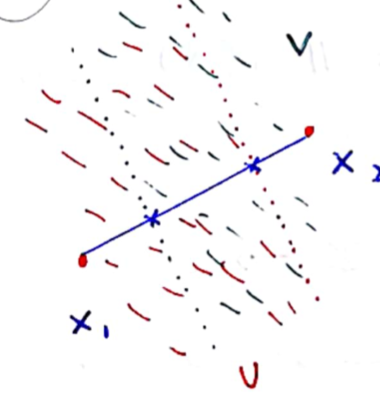
\includegraphics[scale = 0.5]{pictures/exercicimv.png}
        \caption{Representació gràfica de $X$ en $n=2$}
        \label{fig:representaciograficadexexercicimv}
    \end{figure}
    
    Llavors, prenem $U$ com la part vermella de la figura \ref{fig:representaciograficadexexercicimv} i $V$ com la part negra d'aquesta figura. Clarament $U\cap V$ és la part com del mig. Aquí tenim doncs que $X = U\cup V$ i aleshores apliquem Mayer-Vietoris. 
    \begin{equation}
        \notag
        \cdots\rightarrow H_p(U\cap V)\rightarrow H_p(U)\oplus H_p(V)\rightarrow H_p(X)\rightarrow\cdots
    \end{equation}
    Clarament $U\simeq \mathbb{S}^{n-1}$ i el mateix per a $V$. En efecte, doncs $U$ és com un semiplà gegant amb un forat al punt $x_1$ i aleshores retractem tots els punts cap a aquest punt, però sense arribar perquè no existeix. Aleshores obtenim una cosa semblant a una circumferència. Això que explico és amb $n = 2$ eh. Finalment, és clar que $U\cap V$ és $\mathbb{R}^n$ que, de fet, és contràctil, per tant $U\cap V\simeq *$. Amb això tenim ja moltes coses conegudes. Per començar, coneixem $H_p(U)\cong \mathbb{Z}$ per $p=n-1$ i $p = 0$ i $H_p(V)$ el mateix. Aleshores $H_p(U)\oplus H_p(V)\cong\mathbb{Z}\oplus \mathbb{Z}$ per $p=0$ i $p = n-1$, per a la resta és zero. A més, $H_p(U\cap V)\cong\mathbb{Z}$ per $p = 0$ i per la resta és zero. Per tant, quedarà:
    \begin{equation}
        \notag
        \cdots\rightarrow 0\rightarrow H_{n+1}(X)\rightarrow 0\rightarrow0\rightarrow H_n(X)\rightarrow 0\rightarrow\mathbb{Z}\oplus\mathbb{Z}\rightarrow H_{n-1}(X)\rightarrow\cdots
    \end{equation}
    \begin{equation}
        \notag
        \cdots\rightarrow 0\rightarrow H_1(X)\rightarrow \mathbb{Z}\rightarrow \mathbb{Z}\oplus\mathbb{Z}\rightarrow H_0(X)\rightarrow 0
    \end{equation}
    També sabem que $H_0(X)\cong \mathbb{Z}$ en ser $X$ arc-connex. Per tant, la resta són fàcils ja que queden entre successions exactes de termes lliures de torsió. La primera és la següent:
    \begin{equation}
        \notag
        0\rightarrow \mathbb{Z}\oplus\mathbb{Z}\rightarrow H_{n-1}(X)\rightarrow 0
    \end{equation}
    que com té dos termes, és un isomorfisme per ser exacta, és a dir, $H_{n-1}(X)\cong \mathbb{Z}\oplus\mathbb{Z}$. La segona sub-cadena que queda és
    \begin{equation}
        \notag
        0\rightarrow H_1(X)\rightarrow \mathbb{Z}\rightarrow\mathbb{Z}\oplus\mathbb{Z}\rightarrow \mathbb{Z}\rightarrow 0
    \end{equation}
    que, si anomeno $r$ al rang de $H_1(X)$, obtinc l'equació
    \begin{equation}
        \notag
        r-1+2-1=0
    \end{equation}
    que ens dona $r = 0$ i per tant $H_1(X)\cong 0$. Obtenim doncs, 
    \begin{equation}
        \notag
        H_p(X)\cong\left\{
        \begin{array}{ll}
            \mathbb{Z}\oplus\mathbb{Z} & \text{si $p = n-1$}, \\
            0 & \text{si $p\not=n-1$ i $p\not=0$}\\
            \mathbb{Z} & \text{si $p=0$}.
        \end{array}
        \right.
    \end{equation}
    \item Fem el cas general. És molt similar al d'abans, de fet. Agafem els mateixos oberts d'abans, amb $U$ contenint $x_1,\ldots,x_{m-1}$ i $V$ contenint $x_m$. Aleshores veiem que $U\simeq V\simeq X\setminus\{x_1,\ldots,x_{m-1}\}$ i $U\cap V\simeq\mathbb{R}^n\simeq *$. Així doncs, és clar que $V\simeq \mathbb{R}^n\setminus\{x_m\}\simeq \mathbb{S}^{n-1}$ anàlogament al d'abans i aleshores $H_p(V)=H_p(\mathbb{S}^{n-1})$ $\forall p\geq 0$. A més, tenim $H_p(U)$ de forma inductiva. També tenim $H_p(U\cap V) = 0$ per tot $p>0$ per ser contràctil i $H_0(U\cap V)\cong\mathbb{Z}$. Llavors la successió exacta de Mayer Vietoris és una cosa similar a
    \begin{equation}
        \notag
        \cdots\rightarrow 0\rightarrow\mathbb{Z}^m\rightarrow H_{n-1}(X)\rightarrow 0\rightarrow\cdots
    \end{equation}
    \begin{equation}
        \notag
        \cdots\rightarrow 0\rightarrow H_1(X)\rightarrow \mathbb{Z}\rightarrow \mathbb{Z}\oplus\mathbb{Z}\rightarrow H_0(X)\rightarrow 0
    \end{equation}
    on $H_0(X)\cong\mathbb{Z}$ perquè és arc-connex. Seguint els raonaments anàlegs al cas $m = 2$ obtenim $H_1(X) \cong 0$, $H_0(X)\cong\mathbb{Z}$, $H_{n-1}(X)\cong\mathbb{Z}^{\oplus m}$ i $H_p(X)\cong 0$.
\end{enumerate}
\end{sol}






\begin{exercici}
\index{Homologia singular de l'Ampolla de Klein} Calcular l'homologia singular de l'Ampolla de Klein $\mathbb{K}^2$.
\end{exercici}
\begin{sol}
Considerem $X = \mathbb{K}^2$ que surt d'identificar \ref{fig:kleinex} segons indica la figura.
\begin{figure}[H]
    \centering
    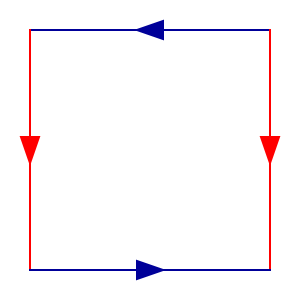
\includegraphics[scale = 0.25]{pictures/kleinbottle.png}
    \caption{Ampolla de Klein sense fer les identificacions}
    \label{fig:kleinex}
\end{figure}
Prenem els següents oberts (figura \ref{fig:obertsklein})
\begin{figure}[H]
    \centering
    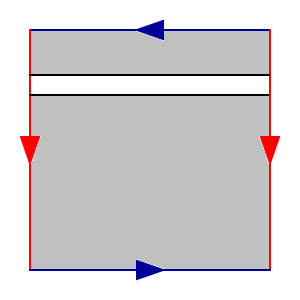
\includegraphics[scale = 0.25]{pictures/kleinU.png}
    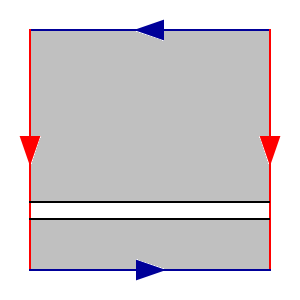
\includegraphics[scale = 0.25]{pictures/kleinV.png}
    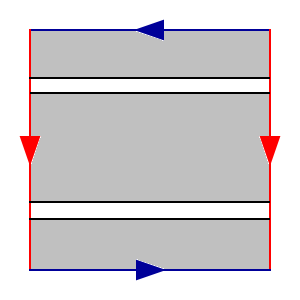
\includegraphics[scale = 0.25]{pictures/kleinUcapV.png}
    \caption{Oberts $U$, $V$ i $U\cap V$ de $\mathbb{K}$}
    \label{fig:obertsklein}
\end{figure}
i és clar que $\mathbb{K}^2 = U\cup V$ i $U\cap V$ és el que he dibuixat. Observem que, retractant com és degut, podem arribar a $U\simeq \mathbb{S}^1$, $V\simeq \mathbb{S}^1$ i $U\cap V\simeq \mathbb{S}^1\sqcup \mathbb{S}^1$. No faig els dibuixos perquè em fa mandra, però amb uns dibuixos es veu prou clar. Tenim la següent successió llarga de Mayer-Vietoris:
\begin{equation}
    \notag
    \cdots 0\rightarrow H_2(\mathbb{K}^2)\overset{\partial_2}{\rightarrow}H_1(U\cap V)\overset{\phi}{\rightarrow} H_1(U)\oplus H_1(V)\overset{\pi}{\rightarrow} H_1(\mathbb{K}^2)\rightarrow
\end{equation}
\begin{equation}
    \notag
    \rightarrow H_0(U\cap V)\rightarrow H_0(U)\oplus H_0(V)\rightarrow H_0(\mathbb{K}^2)\rightarrow 0
\end{equation}
on observem que $H_p(\mathbb{K}^2)\cong 0$ per $p>2$: en efecte, doncs $H_p(\mathbb{S}^1)\cong \mathbb{Z}$ per $p = 0$ i $p = 1$ i per $p \geq 2$ és $H_p(\mathbb{S}^1)\cong 0$ i aleshores la successió llarga de Mayer Vietoris per a $p>2$ és
\begin{equation}
    \notag
    \cdots\rightarrow 0\rightarrow 0\rightarrow H_p(\mathbb{K}^2)\rightarrow 0\rightarrow0\rightarrow\cdots
\end{equation}
i per tant $H_p(\mathbb{K}^2) =0$ per $p>2$. Veiem per $p = 2,1,0$. Per $p = 0$ podem dir que al ser arc-connex, $H_0(\mathbb{K}^2) \cong \mathbb{Z}$. Ara, per calcular $H_1(\mathbb{K}^2)$ i $H_2(\mathbb{K}^2)$ podem separar la successió llarga a partir del morfisme que he anomenat $\phi$ de la següent manera:
\begin{equation}
    \notag
    0\longrightarrow H_2(\mathbb{K}^2)\overset{\partial_2}{\longrightarrow} H_1(U\cap V)\longrightarrow \mathrm{Im}(\phi)\longrightarrow 0
\end{equation}
Llavors, aquí tenim una successió curta exacta i, per tant, $H_2(\mathbb{K}^2)\cong\ker\phi$ ja que $\mathrm{Im}\partial_2 = \ker\phi$ per l'exactitud i de la mateixa manera $\mathrm{Im}\partial_2\cong H_2(\mathbb{K}^2)$ perquè $\partial_2$ és injectiva, al provenir d'un zero cap a $H_2(\mathbb{K}^2)$ i ser la successió exacta (ha de ser $\mathrm{im}0 = \ker(\partial_2) = 0$). Llavors, tenim que $H_2(\mathbb{K}^2)\cong\ker\phi$.

Fem ara un altre tall de la successió llarga, aquest cop per $\pi$ i obtenim la següent successió:
\begin{equation}
    \notag
    0\rightarrow \mathrm{Im}\pi\rightarrow H_1(\mathbb{K}^2)\rightarrow H_0(U\cap V)\rightarrow H_0(U)\oplus H_0(V)\rightarrow H_0(\mathbb{K}^2)\rightarrow 0
\end{equation}
Al posar $\mathrm{Im}\pi$ obtinc el zero de l'esquerra de tot, ja que $\mathrm{Im}\pi\hookrightarrow H_1(\mathbb{K}^2)$ s'injecta. Ara, el primer teorema d'isomorfia em donarà
\begin{equation}
    \notag
    \mathrm{Im}\pi\cong \frac{H_1(U)\oplus H_1(V)}{\ker\pi}
\end{equation}
i per exactitud tenim $\ker\pi\cong \mathrm{Im}\phi$, ergo tenim 
\begin{equation}
    \notag
    \mathrm{Im}\pi\cong \frac{H_1(U)\oplus H_1(V)}{\mathrm{Im}\phi}
\end{equation}
Per tant, si estudiem el morfisme $\phi$ tindrem més pistes sobre $H_1(\mathbb{K}^2)$ i obtindrem $H_2(\mathbb{K}^2)$.

Estudiem doncs el morfisme $\phi:H_1(U\cap V)\longrightarrow H_1(U)\oplus H_1(V)$. Sabem que $U\cap V\simeq \mathbb{S}^1\sqcup\mathbb{S}^1$ i aleshores $H_1(U\cap V)\cong\mathbb{Z}\oplus \mathbb{Z}$. Trobem generadors (figura \ref{fig:kleinmv1}):
\begin{figure}[H]
    \centering
    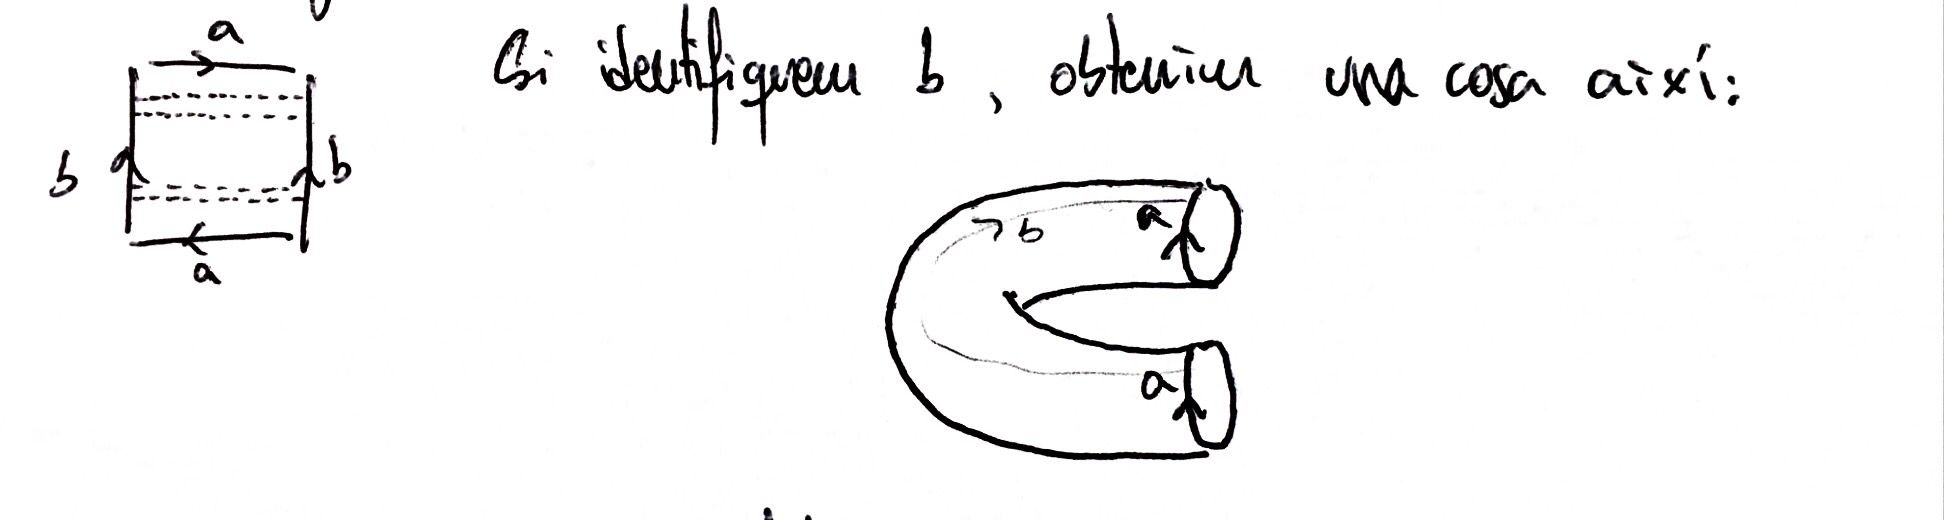
\includegraphics[scale = 0.25]{pictures/kleinmv1.jpeg}
    \caption{Si identifiquem $b$, obtenim una cosa així}
    \label{fig:kleinmv1}
\end{figure}
Llavors, si després identifiquem $a$, en $U\cap V$ queden dos cilindres oberts, un dels quals contenint $a$ i l'altre conté la franja com del mig del quadrat inicial. Per tant, si fico allà un altre camí $c$ tinc la figura \ref{fig:kleinmv2}
\begin{figure}[H]
    \centering
    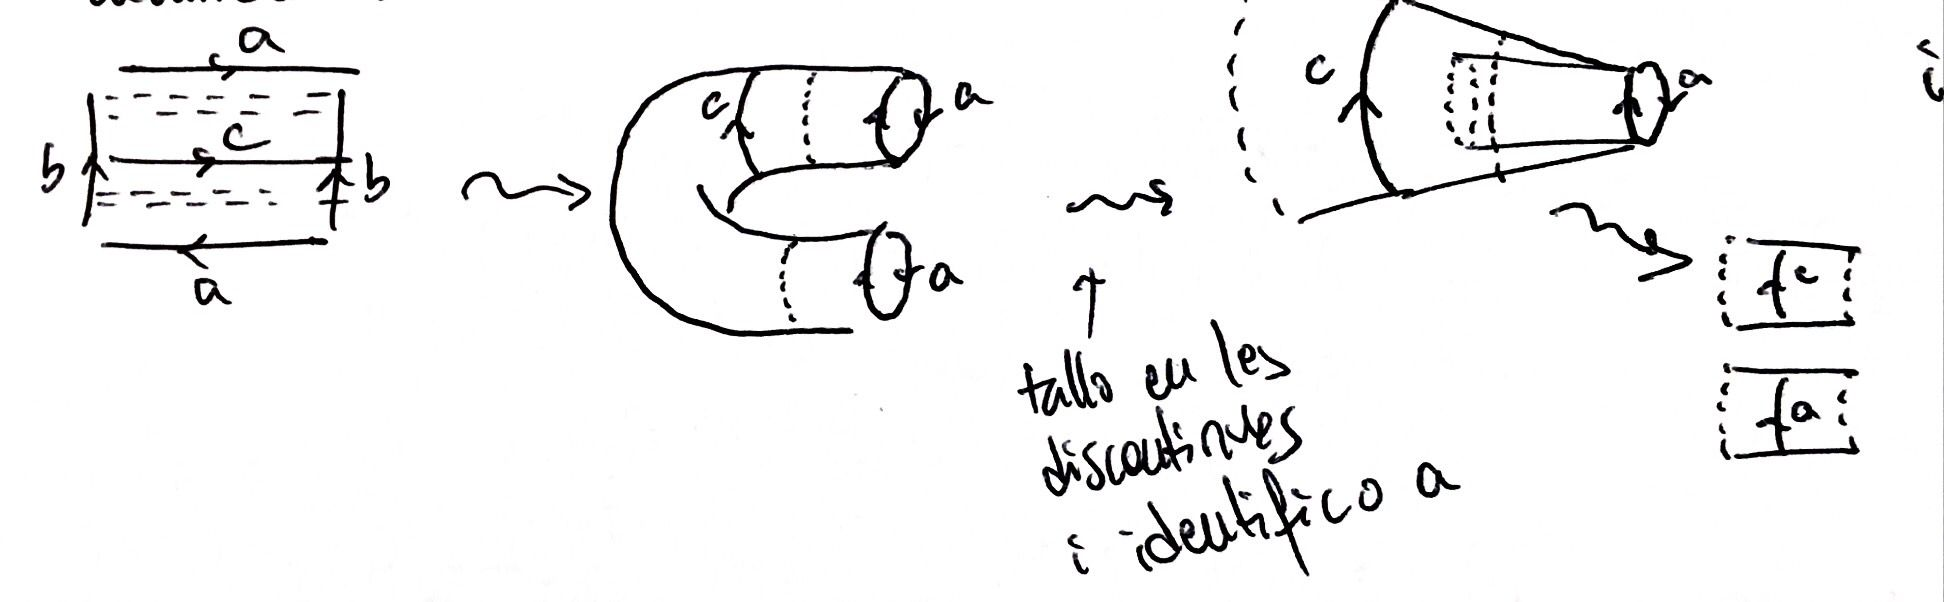
\includegraphics[scale = 0.25]{pictures/kleinmv2.jpeg}
    \caption{Retracte de deformació de $U\cap V$}
    \label{fig:kleinmv2}
\end{figure}
i veiem que al fer retracte de deformació de $U\cap V$ en $\mathbb{S}^1\sqcup\mathbb{S}^1$ obtinc una $\mathbb{S}^1$ generada per $a$ i l'altra per $c$. Per tant, ja tinc dos generadors.

Veiem ara què els hi passa quan fem $\phi$. El dibuix d'abans ho representava molt bé. Veiem on va a parar $c$ en $U$ (figura \ref{fig:kleinmv3})
\begin{figure}[H]
    \centering
    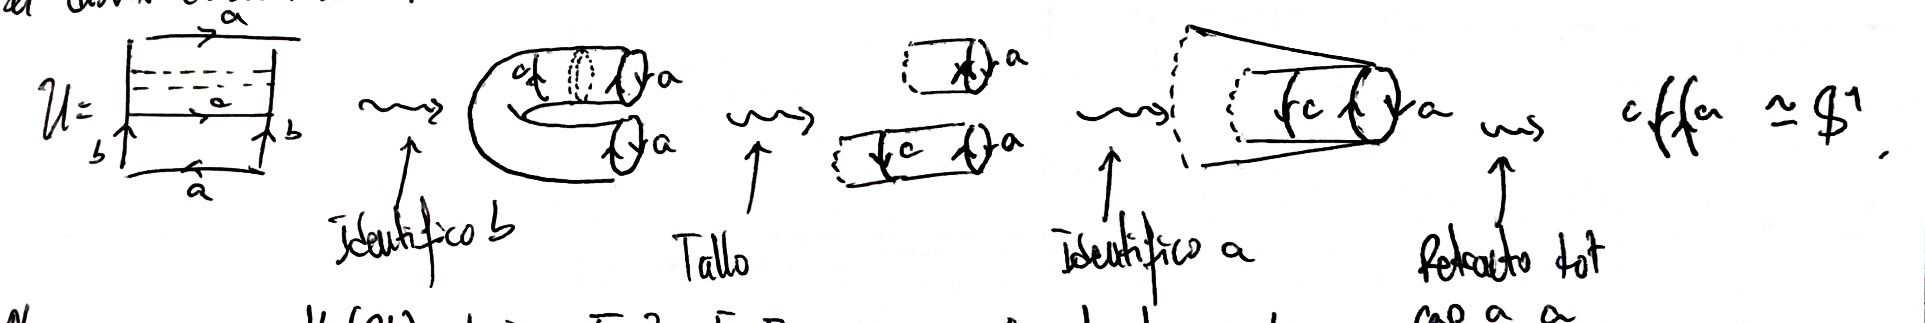
\includegraphics[scale = 0.25]{pictures/kleinmv3.jpeg}
    \caption{Classe de la imatge de $c$ en $H_1(U)$}
    \label{fig:kleinmv3}
\end{figure}
Observem que en $H_1(U)$ tenim $[a] = -[c]$ ja que al retractar sobre $a$ tot $U$, obtinc que els dos camins s'ajunten però en sentit contrari, en una $\mathbb{S}^1$. En $V$ en canvi (figura \ref{fig:kleinmv4})
\begin{figure}[H]
    \centering
    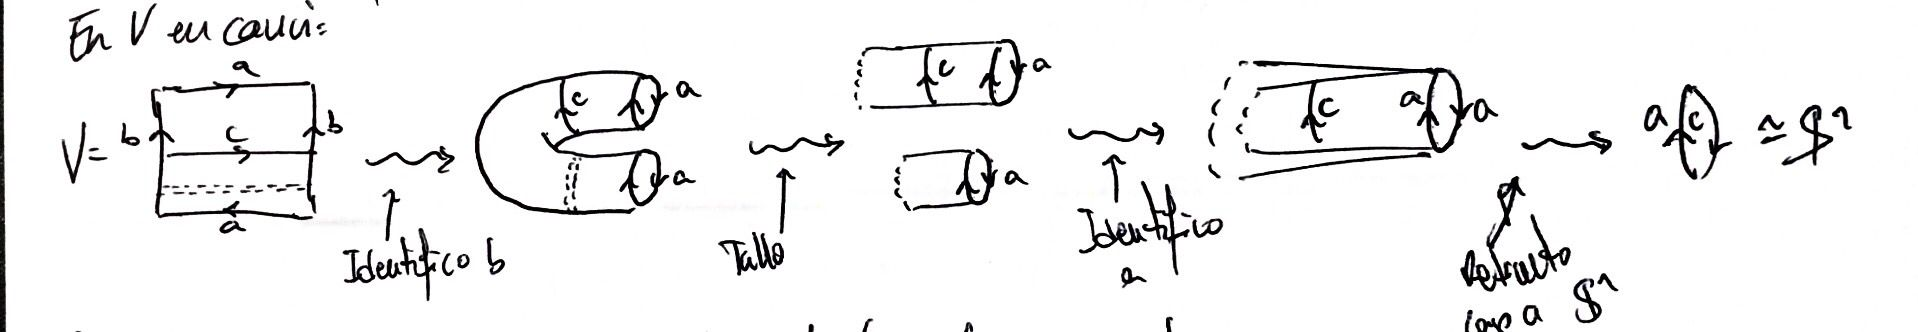
\includegraphics[scale = 0.25]{pictures/kleinmv4.jpeg}
    \caption{Classe de la imatge de $c$ en $H_1(V)$}
    \label{fig:kleinmv4}
\end{figure}
Aquí els dos camins van a parar a $\mathbb{S}^1$ amb la mateixa orientació, ergo en $H_1(V)$ tenim $[a] = [c]$.

Per tant, ja sabem les imatges de $[a]$ i $[c]$ pel morfisme $\phi$:
\begin{equation}
    \notag
    \begin{array}{rl}
        \phi:H_1(U\cap V) & \longrightarrow H_1(U)\oplus H_1(V) \\
        \left[a\right] & \longmapsto (\left[a\right],\left[a\right])\\
        \left[c\right] & \longmapsto (\left[c\right],\left[c\right]) = (-\left[a\right],\left[a\right])
    \end{array}
\end{equation}
i així, $\phi$ té la matriu $M = \left(\begin{smallmatrix}1&-1\\1&1\end{smallmatrix}\right)$. Calculem nucli i imatge i obtenim $\ker\phi = 0$ i $\mathrm{Im}\phi = \langle(1,-1),(1,1)\rangle$ que són linealment independents.

Llavors, seguim amb el problema. Ja hem vist quin era $\ker\phi$ i per tant $H_2(\mathbb{K}^2)\cong 0$. Ara també sabem quina és la imatge de $\phi$ i per tant tenim
\begin{equation}
    \notag
    \frac{H_1(U)\oplus H_1(V)}{\mathrm{Im}\phi}\cong\frac{\mathbb{Z}\oplus\mathbb{Z}}{\langle(-1,1),(1,1)\rangle}\cong\frac{\mathbb{Z}\oplus\mathbb{Z}}{\langle (1,1),(2,0)\rangle}
\end{equation}
ara, a dalt podem escollir generadors de $\mathbb{Z}$ en cada cas de la següent forma:
\begin{equation}
    \notag
    \cong\frac{\mathbb{Z}(1,1)\oplus\mathbb{Z}(1,0)}{\mathbb{Z}(1,1)\oplus\mathbb{Z}(2,0)}\cong\frac{\mathbb{Z}(1,0)}{2\mathbb{Z}(1,0)}\cong\mathbb{Z}/2\mathbb{Z}
\end{equation}
i d'aquesta manera, la successió que teníem curta quedarà
\begin{equation}
    \notag
    0\rightarrow\mathbb{Z}/2\mathbb{Z}\rightarrow H_1(\mathbb{K}^2)\rightarrow \mathbb{Z}\oplus\mathbb{Z}\rightarrow\mathbb{Z}\oplus\mathbb{Z}\rightarrow \mathbb{Z}\rightarrow 0 
\end{equation}
i així, $H_1(\mathbb{K}^2)\cong\mathbb{Z}\oplus\mathbb{Z}/2\mathbb{Z}$.
\end{sol}


\subsection*{Resum del càlcul de grups d'homologia d'alguns espais famosos}

\begin{prop}
[Homologia singular d'espais coneguts]\index{Homologia singular d'espais coneguts} Els càlculs anteriors i altres càlculs que hem fet al llarg del curs donen pas a les següents homologies singulars:
\begin{enumerate}[(a)]
    \item Si $X$ i $Y$ són del mateix tipus d'homotopia, aleshores $H_p(X)\cong H_p(Y)$.
    \item Si $X$ és contràctil, $H_0(X)\cong \mathbb{Z}$ i $H_p(X)\cong 0$ per $p\geq 1$.
    \item Si $X$ és arc-connex, aleshores $H_0(X)\cong\mathbb{Z}$.
    \item Si $X$ és fitat i convex, aleshores $H_p(X) = 0$ per $p>0$.
    \item L'homologia singular de l'esfera $\mathbb{S}^n$ ve donada per
    \begin{equation}
        \notag
        H_p(\mathbb{S}^n)\cong\left\{
        \begin{array}{ll}
            \mathbb{Z}, & \text{si $p = 0$ o $p = n$}\\
            0, & \text{altrament}
        \end{array}
        \right.
    \end{equation}
    \item $H_p(\mathbb{Q})\cong 0$ per $p>0$ i $H_0(\mathbb{Q})\cong\mathbb{Z}^{\oplus|\mathbb{Q}|}$ on $\oplus|\mathbb{Q}|$ a l'exponent de $\mathbb{Z}$ representa que és la suma de $\mathbb{Z}$ indexada per tots els elements de $\mathbb{Q}$.
    \item $\Tilde{H}_0(X)\cong \mathbb{Z}^{\oplus r}$, on $r$ és el nombre de components arc-connexes de $X$. Aleshores $H_0(X)$ és afegir una $\mathbb{Z}$ a això. D'altra banda $\Tilde{H}_p(X)\cong H_p(X)$ per $p\geq 1$.
    \item $\Tilde{H}_0(X_1\vee X_2)\cong \Tilde{H}_0(X_1)\oplus \Tilde{H}_0(X_2)$ però no és cert per $H_0$ normal. En canvi, per $n\geq 1$ sí que és cert $H_n(X_1\vee X_2)\cong H_n(X_1)\oplus H_n(X_2)$.
    \item $H_p(X\times\mathbb{S}^n)\cong H_{p-1}(X)\oplus H_p(X)$, per $p\geq 0$.
\end{enumerate}
\end{prop}



\section{Homologia relativa singular}
En aquest apartat estudiarem les parelles d'espais topològics formades per un espai topològic $X$ i un subespai $A$ de $X$, direm aleshores que $(X,A)$ és un parell topològic. Si $(X,A)$ i $(Y,B)$ són parells topològics, una aplicació contínua de parells $f:(X,A)\rightarrow (Y,B)$ és una aplicació contínua $f:X\rightarrow Y$ tal que $f(A)\subset B$. És immediat comprovar que els parells topològics i les aplicacions de parells formen una categoria, que notarem $\mathbf{Top}^2$.

L'aplicació d'inclusió $i:A\hookrightarrow X$ és una aplicació contínua i, per tant, indueix un morfisme de complexos de cadenes singulars
\begin{equation}
    \notag
    \begin{array}{rl}
        S_\bullet(i):S_\bullet(A) & \longrightarrow S_\bullet(X) \\
        \sigma & \longmapsto\sigma
    \end{array}
\end{equation}
que és injectiu.

\begin{defi}
El \textit{complex de cadenes singulars relatives del parell $(X,A)$}, que denotarem per $S_\bullet(X,A)$, és el complex quocient $S_\bullet(X)/S_\bullet(A)$, és a dir,
\begin{equation}
    \notag
    S_p(X,A):=\frac{S_p(X)}{S_p(A)},
\end{equation}
per a tot $p\geq 0$. Es defineix l'\textit{homologia relativa del parell $(X,A)$}\index{Homologia relativa del parell $(X,A)$}, que denotarem per $H_\bullet(X,A)$, com l'homologia del complex $S_\bullet(X,A)$, és a dir,
\begin{equation}
    \notag
    H_\bullet(X,A):=H_\bullet(S_\bullet(X,A)) = H_\bullet\left(\frac{S_\bullet(X)}{S_\bullet(A)}\right).
\end{equation}  
\end{defi}

Els grups $S_p(X,A)$ són grups abelians lliures, ja que són isomorfs als subgrups de $S_p(X)$ generats per tots els $p$-símplexs singulars no continguts en $A$.

\begin{prop}
Siguin $(X,A)$, $(Y,B)$ parells topològics i $f:(X,A)\rightarrow (Y,B)$ una aplicació contínua de parells. Aleshores $f$ indueix un morfisme natural en homologia relativa
\begin{equation}
    \notag
    H_\bullet(f):H_\bullet(X,A)\rightarrow H_\bullet(Y,B),
\end{equation}
tal que, si $\sigma$ és un cicle relatiu, aleshores $H_\bullet(f)(\sigma) = [S_\bullet(f)(\sigma)]$. A més a més, l'homologia relativa indueix un functor
\begin{equation}
    \notag
    H_\bullet:\mathbf{Top}^2\longrightarrow \mathbf{Ab}.
\end{equation}  
\end{prop}
\begin{proof}
Per definició
\begin{equation}
    \notag
    S_\bullet(X,A):=S_\bullet(X)/S_\bullet(A),\qquad S_\bullet(Y,B):=S_\bullet(Y)/S_\bullet(B).
\end{equation}
L'aplicació $f$ indueix un morfisme de complexos que per la functorialitat de $S_\bullet$ fan commutatiu el diagrama
\begin{equation}
    \notag
    \xymatrix{
    S_\bullet(A)\ar[r]^{S_\bullet(f)}\ar[d]_{S_\bullet(i)} & S_\bullet(B)\ar[d]^{S_\bullet(i)}\\
    S_\bullet(X)\ar[r]^{S_\bullet(f)} & S_\bullet(Y).
    }
\end{equation}
Així, per pas al quocient, resulta el diagrama commutatiu de les successions exactes
\begin{equation}
    \notag
    \xymatrix{
    0\ar[r]&S_\bullet(A)\ar[r]\ar[d]_{S_\bullet^{A}} & S_\bullet(X)\ar[r]\ar[d]_{S_\bullet^X}& S_\bullet(X,A)\ar[r]\ar[d]_{S_\bullet^{(X,A)}} & 0\\
    0\ar[r] & S_\bullet(B)\ar[r] & S_\bullet(Y)\ar[r] & S_\bullet(Y,B)\ar[r] & 0
    }
\end{equation}
El morfisme de complexos $S_\bullet^{(X,A)}(f)$ indueix el morfisme en homologia buscat. La functorialitat és immediata a partir de la functorialitat de $S_\bullet^{(X,A)}$.
\end{proof}

\begin{ter}
Si $(X,A)$ és un parell topològic, llavors hi ha una successió exacta llarga
\begin{equation}
    \notag
    \cdots\longrightarrow H_p(A)\overset{i_\bullet}{\longrightarrow} H_p(X)\overset{\pi_\bullet}{\longrightarrow} H_p(X,A)\overset{\partial_\bullet}{\longrightarrow} H_{p-1}(A)\longrightarrow \cdots
\end{equation}
que s'anomena la \textit{successió exacta d'homologia relativa del parell $(X,A)$}. Aquesta successió exacta és natural en el parell $(X,A)$, és a dir, si $f:(X,A)\rightarrow (Y,B)$ és una aplicació contínua de parells, aleshores el diagrama de successions exactes
\begin{equation}
    \notag
    \xymatrix{
    \cdots\ar[r] & H_p(A)\ar[r]^{i_\bullet}\ar[d] & H_p(X)\ar[r]^{\pi_\bullet}\ar[d] & H_p(X,A)\ar[r]^{\partial_\bullet}\ar[d] & H_{p-1}(A)\ar[r]\ar[d] & \cdots \\
    \cdots\ar[r] & H_p(B)\ar[r]^{j_\bullet}\ar[r]& H_p(Y)\ar[r]^{\pi_\bullet'} & H_p(Y,B)\ar[r]^{\partial_\bullet} & H_{p-1}(B)\ar[r] & \cdots
    }
\end{equation}
és commutatiu.
\end{ter}
\begin{proof}
Per la definició del complex singular relatiu $S_\bullet(X,A)$, tenim la successió exacta de complexos
\begin{equation}
    \notag
    0\longrightarrow S_\bullet(A)\overset{S_\bullet(i)}{\longrightarrow} S_\bullet(X)\overset{S_\bullet(\pi)}{\longrightarrow} S_\bullet(X,A)\longrightarrow 0,
\end{equation}
i per no sé quin teorema s'obté la successió exacta llarga d'homologia ssociada
\begin{equation}
    \notag
    \cdots \longrightarrow H_p(A)\overset{i_\bullet}{\longrightarrow} H_p(X)\overset{\pi_\bullet'}{\longrightarrow} H_p(X,A)\overset{S_\bullet(\pi)}{\longrightarrow} S_\bullet(X,A)\longrightarrow \cdots
\end{equation}
Si $f:(X,A)\rightarrow (Y,B)$ és una aplicació contínua de parells, aleshores el diagrama de successions exactes de complexos
\begin{equation}
    \notag
    \xymatrix{
    0\ar[r] & S_\bullet(A)\ar[d]\ar[r] & S_\bullet(X)\ar[d]\ar[r] & S_\bullet(X,A)\ar[r]\ar[d] & 0 \\
    0 \ar[r] & S_\bullet(B)\ar[r] & S_\bullet(Y)\ar[r] & S_\bullet(Y,B)\ar[r] & 0
    }
\end{equation}
és commutatiu, així de (??) resulta la naturalitat de la successió exacta d'un parell.
\end{proof}


Hi ha una noció d'homotopia de parelles. 
\begin{defi}
Donades $f,g:(X,A)\rightarrow (Y,B)$ direm que $f$ i $g$ són homòtopes en $\mathbf{Top}_2$ (o homòtopes mòdul $A$) si existeix
\begin{equation}
    \notag
    F:(X\times [0,1],A\times [0,1])\rightarrow Y\times B
\end{equation}
tal que $F(x,0) = f(x)$ i $F(x,1) = g(x)$, $\forall x\in X$.
\end{defi}


\begin{nota}
$f,g:X\rightarrow Y$, $A\subset X$, teníem la noció d'aplicacions homotòpicament equivalents, $f\sim_A g$. Però aquella noció no és idèntica al que hem definit. La definició actual d'homotopia implica la definició anterior.
\end{nota}

\begin{ter}
[Invariància homotòpica de parelles]\label{ter:invarianciahomotopicadeparelles} Si $f,g:(X,A)\rightarrow (Y,B)$ homòtopes en $\mathbf{Top}_2$, aleshores
\begin{equation}
    \notag
    f_\bullet = g_\bullet:H_p(X,A)\longrightarrow H_p(Y,B),\quad \forall p\geq 0  
\end{equation}
\end{ter}
\begin{proof}
Sigui $i:A\hookrightarrow X$. És fàcil veure que l'homotopia que vam construir en el cas absolut és funcional. En el nostre cas
\begin{equation}
    \notag
    \xymatrix{
    S_p(A)\ar[d]^{i_\bullet} \ar[r]^{h_p^{A}}&  S_{p+1}(A\times [0,1])\ar[d]^{i_\bullet\times \mathrm{id}} &  \lambda_0^{A}\overset{h_p^{A}}{\sim} \lambda_1^{A}\\
    S_p(X) \ar[r]_{h_p^X} & S_{p+1}(X\times [0,1]) & \lambda_0^X\overset{h_p^X}{\sim}\lambda_1^X
    }
\end{equation}
Fent servir aquesta homotopia com en el cas absolut, s'obté $f_\bullet = g_\bullet:H_p(X,A)\rightarrow H_p(Y,B)$, $\forall p\geq 0$.
\end{proof}

\section{El teorema d'escissió}

Sigui $X$ un espai topològic, $A\subset X$ i $U\subset A$. Llavors tenim un morfisme de parelles en $\mathbf{Top}_2$
\begin{equation}
    \notag
    (X\setminus U,A\setminus U)\longrightarrow(X,A)
\end{equation}
Es pot interpretar com una simple inclusió de $X\setminus U$ dins de $X$ i el mateix amb $A$. Aquesta aplicació indueix, $\forall p\geq 0$, 
\begin{equation}
    \notag
    H_p(X\setminus U,A\setminus U)\longrightarrow H_p(X,A)\quad \forall p\geq 0
\end{equation}

\begin{defi}
[Escissió]\index{Escissió} Sigui $(X,A)$ un parell topològic i $U$ un subespai de $A$. Es diu que $U$ és \textit{escissió} en $(X,A)$\index{Escissió} si el morfisme $H_\bullet(X\setminus U,A\setminus U)\rightarrow H_\bullet(X,A)$ induït per la inclusió, és un isomorfisme.
\end{defi}

\begin{ter}
[Teorema d'escissió]\index{Teorema d'escissió}\label{ter:teoremaescissio} Sota les mateixes hipòtesis, si es verifica $\overline{U}\subset\overset{\circ}{A}$, aleshores 
\begin{equation}
    \notag
    H_p(X\setminus U, A\setminus U) \longrightarrow H_p(X,A)
\end{equation}
és isomorfisme $\forall p\geq 0$. Es diu que $U$ és \textit{escissió} en $(X,A)$\index{Escissió}.
\end{ter}
\begin{proof}
Considerem el recobriment de $X$, $\mathcal{U} = \{A,X\setminus U\}$. Aleshores podem reescriure $X$ així:
\begin{equation}
    \notag
    X = \overline{U}\cup(X\setminus \overline{U}) = \overset{\circ}{A}\cup(X\setminus\overline{U}) = \overset{\circ}{A}\cup(X\setminus U)^\circ
\end{equation}
Per tant, $S_\bullet(\mathcal{U})\rightarrow S_\bullet(X)$ indueix un isomorfisme en homologia (pel Teorema de les Cadenes Petites, \ref{ter:cadenespetites}). 

Considerem
\begin{equation}
    \notag
    \xymatrix{
    0 \ar[r] & S_\bullet(\{A,A\setminus U\}) \ar[r]\ar[d] & S_\bullet(\{A,X\setminus U\}) \ar[r]\ar[d] & \frac{S_\bullet(\{A,X\setminus U\})}{S_\bullet(\{A,A\setminus U\})} \ar[r]\ar[d] & 0 \\
    0 \ar[r] & S_\bullet(A)\ar[r] & S_\bullet(X) \ar[r] & S_\bullet(X,A) \ar[r] & 0
    }
\end{equation}
Tenim
\begin{equation}
    \notag
    \xymatrix{
    H_p(A) \ar[r]\ar[d] & H_p(\{A,X\setminus U\}) \ar[r]\ar[d] & H_p\left(\frac{S_\bullet(\{A,X\setminus U\})}{S_\bullet(\{A,A\setminus U\})}\right) \ar[r]\ar[d] & H_{p-1}(A) \ar[r]&\cdots \\
    H_p(A)\ar[r] & H_p(X) \ar[r] & H_p(X,A) \ar[r] & H_{p-1}(A) \ar[r]&\cdots
    }
\end{equation}
Llavors, pel lema dels 5,
\begin{equation}
    \notag
    H_p\left(\frac{S_\bullet(\{A,X\setminus U\})}{S_\bullet(\{A,X\setminus U\})}\right) \cong H_p(X,A)
\end{equation}
Ara, pel lema dels 9, tenim el següent diagrama
\begin{equation}
    \notag
    \xymatrix{
     & 0\ar[d] & 0\ar[d] & 0\ar[d] & \\
     0\ar[r] & S_\bullet(A\setminus U)\ar[r]\ar[d] & S_\bullet(A\setminus U) \ar[r]\ar[d] & 0\ar[r]\ar[d] & 0 \\
     0\ar[r] & S_\bullet(A)\oplus S_\bullet(A\setminus U) \ar[d]\ar[r] & S_\bullet(A)\oplus S_\bullet(X\setminus U) \ar[r]\ar[d] & \frac{S_\bullet(X\setminus U)}{S_\bullet(A\setminus U)} \ar[d]\ar[r] & 0 \\
     0 \ar[r] & S_\bullet(\{A,A\setminus U\})\ar[r]\ar[d] & S_\bullet(\{A,X\setminus U\})\ar[d]\ar[r] & \frac{S_\bullet(A,X\setminus U)}{S_\bullet(A,A\setminus U)}\ar[r]\ar[d] & 0 \\
     & 0& 0 & 0 &
    }
\end{equation}
Totes les files són exactes (es pot comprovar fàcilment) i les dues primeres columnes també són exactes. Faltaria demostrar que la tercera columna és exacta, i aleshores tindrem l'isomorfisme desitjat, ja que si tenim una successió exacta $0\rightarrow A\rightarrow B\rightarrow 0$, on $f:A\rightarrow B$, aleshores $f$ és isomorfisme perquè $\ker 0 = \mathrm{Im}f$ i $\ker f = \mathrm{Im}0$, la primera implica exhaustivitat i la segona injectivitat. Així doncs, tenim l'isomorfisme
\begin{equation}
    \notag
    \frac{S_\bullet(X\setminus U)}{S_\bullet(A\setminus U)}\cong \frac{S_\bullet(A,X\setminus U)}{S_\bullet(A,A\setminus U)}
\end{equation}
Llavors, la homologia del primer, que és $H_p(X\setminus U, A\setminus U)$ és isomorfa a la homologia del segon, que és la que teníem abans que era isomorfa a $H_p(X,A)$. Per tant, es compleix l'isomorfisme $H_p(X\setminus U,A\setminus U)\cong H_p(X,A)$.
\end{proof}


\begin{exercici}
[Fórmula equivalent del teorema d'escissió] Si $X$ és un espai topològic, $V,W\subset X$ tals que $X = \overset{\circ}{U}\cup\overset{\circ}{V}$, aleshores
\begin{equation}
    \notag
    (V,V\cap W)\hookrightarrow (X,W)
\end{equation}
indueix un isomorfisme de grups $H_p(V,V\cap W)\rightarrow H_p(X,W)$, $\forall p\geq 0$.
\end{exercici}

\begin{ej}
Sigui $X = \mathbb{S}^2$ i $A = \mathbb{S}^2_+ = \{(x,y,z)\in\mathbb{S}^2\;:\;z\geq 0\}$ i $U = \{(0,0,1)\}$ el pol nord. Com $\overline{U} = U\subset\mathring{A}$, pel teorema d'escissió $U$ és escissiu, i els morfismes
\begin{equation}
    \notag
    H_p(X\setminus U,A\setminus U)\rightarrow H_p(X,A)
\end{equation}
són isomorfismes per $p\geq 0$. En el cas $p = 0$ això és trivial ja que $H_0(X\setminus U,A\setminus U) = H_0(X,A)=0$, però per $p = 1$ es té
\begin{equation}
    \notag
    H_1(X\setminus U,A\setminus U)\cong \mathbb{Z}\qquad H_1(X,A)\cong \mathbb{Z},
\end{equation}
i en aquest cas el fet que el morfisme $H_1(X\setminus U,A\setminus U)\rightarrow H_1(X,A)$ sigui un isomorfisme ja no és una trivialitat.
\end{ej}


\begin{coro}
Sigui $X$ un espai topològic, i $U\subseteq A\subseteq B\subseteq X$ tres subespais de $X$. Si $\overline{U}\subseteq\mathring{B}$ i les inclusions $A\hookrightarrow B$, $A\setminus U\hookrightarrow B\setminus U$ són equivalències homotòpiques, aleshores $U$ és escissió en $(X,A)$.
\end{coro}

\begin{ej}
Sigui $X = \mathbb{S}^2$, $A = \mathbb{S}^2_+$ i $U = \mathbb{E}^2 = \{(x,y,z)\in\mathbb{S}^2$\;:\;z>0\}. Si prenem $B = \mathbb{S}^2\setminus\{(0,0,-1)\}$, tindrem que $\overline{U}\subseteq \mathring{B} = B$ i $A$ i $A\setminus U$ són retractes de deformació de $B$ i $B\setminus U$, respectivament. Podem aplicar doncs el corol·lari anterior i deduir que $U$ és escissió en $(X,A)$.
\end{ej}

\section{Comparació homologia singular i simplicial}

En els apartats anteriors hem anat desenvolupant les propietats bàsiques de l'homologia singular. En aquest apartat anem a veure com aquestes propietats ens permeten comparar l'homologia simplicial d'un políedre amb la seva homologia singular.

Si $K$ és un complex simplicial i $K'\subset K$ és un subcomplex, aleshores definim
\begin{equation}
    \notag
    C_\bullet(K, K') = \frac{C_\bullet(K)}{C_\bullet(K')}
\end{equation}
i l'homologia simplicial del parell $(K,K')$
\begin{equation}
    \notag
    H_p(K,K') := H_p(C_\bullet(K,K'))
\end{equation}
Tenim la cadena
\begin{equation}
    \notag
    0\rightarrow C_\bullet(K')\rightarrow C_\bullet(K)\rightarrow C_\bullet(K,K')\rightarrow 0
\end{equation}
que en dona una successió llarga (exacta)
\begin{equation}
    \notag
    \cdots\rightarrow H_p(K')\rightarrow H_p(K)\rightarrow H_p(K,K')\rightarrow \cdots
\end{equation}

\begin{itemize}
    \item Una cosa que també serà molt útil és el càlcul de l'homologia simplicial d'un símplex. Això està com a exercici a les llistes, però ho resumeixo a continuació. Si $\Delta^n$ és un símplex $n$-dimensional, $C_\bullet(\Delta^n)$ és contràctil en grau $>0$, és a dir,
\begin{equation}
    \notag
    H_p(\Delta^n)= 0, \forall p>0
\end{equation}
S'assembla molt a un resultat que dèia que $\mathbb{R}^n$ que sigui convex i acotat (crec), aleshores la seva homologia singular s'anul·la Es defineixen $h_p:C_p(\Delta^n)\rightarrow C_{p+1}(\Delta^n)$ tal que $\mathrm{id} = \partial h + h\partial$. La sub-$p$ es defineix tal que si $v_0$ és un vèrtex de $\Delta^n$, donat un $\sigma_p = [v_{i_0},\ldots,v_{i_p}]$ es defineix
\begin{equation}
    \notag
    h_p(\sigma_p) = \left\{
    \begin{array}{ll}
        0 & \text{si $v_0\in\{v_{i_0},\ldots,v_{i_p}\}$} \\
        \left[v_0,v_{i_0},\ldots,v_{i_p}\right] & \text{si $v_0\not\in\{v_{i_0},\ldots,v_{i_p}\}$}
    \end{array}
    \right.
\end{equation} on aquí s'ha d'entendre la signatura del símplex ordenat multiplicada pel símplex ordenat.


\item Sigui $K$ un complex simplicial ordenat. Si $s = [v_{i_0},\ldots,v_{i_p}]$ és un símplex de $K$, definim en $|K|$ un símplex singular per
\begin{equation}
    \notag
    \begin{array}{rl}
        \sigma_s:\Delta^p & \longrightarrow |K| \\
        (\lambda_0,\ldots,\lambda_p) & \longmapsto \sum_{j=0}^p\lambda_j v_{i_j}
    \end{array}
\end{equation}
Tenim morfismes
\begin{equation}
    \notag
    \begin{array}{rl}
        C_p(K) & \longrightarrow S_p(|K|) \\
        s & \longmapsto \sigma_s
    \end{array}
\end{equation}
que defineixen morfismes de complexos de cadenes $C_\bullet(K)\rightarrow S_\bullet(|K|)$. Si $K_1\overset{f}{\longrightarrow} K_2$ és simplicial, tenim 
\begin{equation}
    \notag
    |f|:|K_1|\longrightarrow |K_2|
\end{equation}
i es verifica que el diagrama
\begin{equation}
    \notag
    \xymatrix{
    C_\bullet(K_1) \ar[r]^{\varsigma_{K_1}}\ar[d]_f & S_\bullet(|K_1|) \ar[d]^{|f|} \\
    C_\bullet(K_2)\ar[r]^{\varsigma_{K_2}} & S_\bullet(|K_2|)
    }
\end{equation}
és commutatiu.
\end{itemize}



\begin{ter}
Si $K$ és un complex simplicial ordenat, aleshores l'aplicació induïda per $\varsigma_K$
\begin{equation}
    \notag
    H_p^{\mathrm{simp}}(K)\longrightarrow H_p^{\mathrm{sing}}(|K|)    
\end{equation}
és isomorfisme $\forall p\geq 0$.
\end{ter}
\begin{proof}
Per inducció sobre $n = \dim K$.
\begin{enumerate}[(1)]
    \item Si $n= 0$, aleshores $|K|$ és finit (amb la topologia discreta) i 
    \begin{equation}
        \notag
        H_0(K)\longrightarrow H_0(|K|)
    \end{equation}
    és isomorfisme ja que les classes $[v]$ són base a tots dos grups.
    
    \item Suposem donat el resultat per políedres $K$ de dimensió $\dim K<n$ i prenem un políedre $K$ de dimensió $\leq n$. Ara farem inducció sobre el nombre de símplexs de $K$ que tinguin exactament $n$ vèrtexs. Siguin $S_1,\ldots,S_m$ els símplexs $n$-dimensionals de $K$. Fem inducció sobre $m$. 
    
    El pas $m = 0$ és absurd ja que aleshores no hi ha cap símplex $n$-dimensional i per tant s'aplica la hipòtesi d'inducció sobre $n$. En efecte, si $m = 0$, aleshores $\dim K<n$ i s'aplica hipòtesi d'inducció sobre $n$ i ja ho tenim.
    
    Sigui doncs $m>0$ i aleshores sigui $L$ el subcòmplex de $K$ amb les mateixes cares llevat de $S_m$ i que les cares de $S_m$ no siguin comunes amb cap altre símplex de $K$. Tenim
    \begin{equation}
        \notag
        C_p(L) = C_p(K)\qquad p\not =n
    \end{equation}
    i en cas que $p = n$ tenim
    \begin{equation}
        \notag
        C_n(L)=\bigoplus\mathbb{Z}S_i,\quad i=1,\ldots,m-1
    \end{equation}
    
    Llavors tenim el diagrama commutatiu següent
    \begin{equation}
        \notag
        \xymatrix{
        0\ar[r] & C_\bullet(L)\ar[d]^{\nu^L}\ar[r] & C_\bullet(K)\ar[d]^{\nu^K}\ar[r]& C_\bullet(K,L)\ar[d]\ar[r]& 0 \\
        0 \ar[r] & S_\bullet(|L|)\ar[r] & S_\bullet(|K|)\ar[r] & S_\bullet(|K|,|L|)\ar[r] & 0
        }
    \end{equation}
    Les aplicacions horitzontals són les naturals de sempre i les verticals són el morfisme que volem trobar que dona un isomorfisme en homologia, per $L$ i per $K$ respectivament i l'últim el quocient. Aquest diagrama és commutatiu. 
    
    La part horitzontal de dalt dona lloc a una successió llarga d'homologia simplicial i la de sota dona pas a una successió llarga d'homologia singular i ambdues estan connectades. Llavors, per hipòtesis d'inducció, els morfismes $\nu^L$ indueixen isomorfismes entre les homologies simplicial i singular. Llavors, si aconseguim veure que els morfismes $C_\bullet(K,L)\rightarrow S_\bullet(|K|,|L|)$ indueixen isomorfismes en homologia singular i simplicial, tindrem que els $\nu^K$ estan rodejats de morfismes que indueixen isomorfismes en homologies singular i simplicial i, aleshores, ho hauran de ser també pel lema dels cinc. Ho torno a dir més clar.
    
    Si veiem que els morfismes induïts en homologia
    \begin{equation}
        \notag
        H_p^{\mathrm{simp}}(K,L)\rightarrow H_p^{\mathrm{sing}}(|K|,|L|)
    \end{equation}
    són isomorfismes $\forall p\geq 0$, aleshores considerant les successions llargues d'homologia, la hipòtesi d'inducció i el lema dels 5 tindran el resultat que volem.
    
    Considerem el següent quadrat commutatiu:
    \begin{equation}
        \notag
        \xymatrix{
        H_p^{\mathrm{simp}}(S_m,\partial S_m)\ar[r]\ar[d] & H_p^{\mathrm{simp}}(K,L)\ar[d]^\nu\\
        H_p^{\mathrm{sing}}(|S_m|,|\partial S_m|)\ar[r] & H_p^{\mathrm{sing}}(|K|, |L|)
        }
    \end{equation}
    Aquesta aplicació (la horitzontal de dalt) és induïda per $(S_m,\partial S_m)\hookrightarrow(K,L)$; l'aplicació vertical de l'esquerra és la que volem estudiar per $K = S_m$ i $L = \partial S_m$ i l'aplicació horitzontal de sota és la induïda per la inclusió de parelles d'espais topològics $(|S_m|,|\partial S_m|)\hookrightarrow (|K|,|L|)$. Queda com a exercici provar que el quadrat és commutatiu.
    
    Llavors, nosaltres el que volem és mostrar que $\nu$ és isomorfisme, cosa que farem demostrant que les altres ho són. Les numeraré així:
    \begin{equation}
        \notag
        \xymatrix{
        H_p^{\mathrm{simp}}(S_m,\partial S_m)\ar[r]^{(a)}\ar[d]^{(b)} & H_p^{\mathrm{simp}}(K,L)\ar[d]^\nu\\
        H_p^{\mathrm{sing}}(|S_m|,|\partial S_m|)\ar[r]^{(c)} & H_p^{\mathrm{sing}}(|K|, |L|)
        }
    \end{equation}
    per poder fer-ho més clar.
    
    \begin{enumerate}
        \item Mostrem que això és isomorfisme. El complex
        \begin{equation}
            \notag
            C_p(K,L) = \frac{C_p(K)}{C_p(L)}\cong \left\{
            \begin{array}{ll}
                0 & p\not=n \\
                \mathbb{Z}s_n & p = n
            \end{array}
            \right.
        \end{equation}
        i el complex de l'esquerra és, anàlogament,
        \begin{equation}
            C_p(S_m,\partial S_m) = \left\{
            \begin{array}{ll}
                0 & p\not=n \\
                \mathbb{Z}s_n & p = n
            \end{array}
            \right.
        \end{equation}
        i per tant és clar que (a) és un isomorfisme. 
        
        \item Per provar que (b) és un isomorfisme considerarem el següent lema.
        
        \begin{lema}
        Sigui $X$ un espai topològic, $U\subset A\subset B\subset X$ subespais. Anem a suposar primer que $\overline{U}\subset\mathring{B}$, $A\hookrightarrow B$, $A\setminus U\hookrightarrow B\setminus U$ són equivalències homològiques. Aleshores
        \begin{equation}
        \notag
        H_p(X\setminus U,A\setminus U)\longrightarrow H_p(X,A)
        \end{equation}
        és isomorfisme $\forall p\geq 0$.
        \end{lema}
        \begin{proof}
        Tenim
        \begin{equation}
        \notag
        \xymatrix{
        H_p(X\setminus U,A\setminus U)\ar[r]\ar[d] & H_p(X,A)\ar[d]\\
        H_p(X\setminus U,B\setminus U)\ar[r] & H_p(X,B)   
        }
        \end{equation}  
        Es té que $H_p(X\setminus U,A\setminus U)\rightarrow H_p(X\setminus U,B\setminus U)$ és isomorfisme. En efecte,
        \begin{equation}
            \notag
            \xymatrix{
            H_p(A\setminus U)\ar[d]^{\cong}\ar[r] & H_p(X\setminus U)\ar[d]^{\cong}\ar[r] & H_p(X\setminus U, A\setminus U)\ar[r]\ar[d]^{(*)} & H_{p-1}(A\setminus U)\ar[r]\ar[d]^{\cong}& \cdots   \\
            H_p(B\setminus U)\ar[r] & H_p(X\setminus U)\ar[r] & H_p(X\setminus U,B\setminus U)\ar[r] & H_{p-1}(B\setminus U)\ar[r] & \cdots
            }
        \end{equation}
        i pel lema dels 5 més la hipòtesis, tenim que és isomorfisme. Ara, $H_p(X\setminus U,B\setminus U)\rightarrow H_p(X,B)$ també és isomorfisme per escissió. Per tant, finalment, $H_p(X,A)\rightarrow H_p(X,B)$ és isomorfisme com volíem veure.
        \end{proof}
        
        Continuem amb la demostració. Aplicarem aquest lema a la nostra situació. Sigui $b_m$ el baricentre de $S_m$. Siguin $A = |L|$, $B = |K|\setminus\{b_m\}$, $X = |K|$, $U = |K|\setminus|S_m|$. Tenim doncs, $A\hookrightarrow B$ equivalència homològica (de fet, és una retracció de $|S_m|\setminus\{b_m\}$ sobre $|\partial S_m|$); $A\setminus U\hookrightarrow B\setminus U$ també és equivalència homològica ja que $|\partial S_m|\hookrightarrow |S_m|\setminus \{b_m\}$ fent una retracció com abans; finalment, $\overline{U}\subset\mathring{B}=B$ (ja que $B$ és obert) és clar perquè $|L|\subset |K|\setminus\{b_m\}$. Aplicant el lema doncs, tenim que 
        \begin{equation}
            \notag
            H_p(|S_m|,|\partial S_m|)\overset{\cong}{\longrightarrow} H_p(|K|,|L|)
        \end{equation}
        que és el que volíem. 

        \item Demostrem ara que (c) és isomorfisme. Tenim 
        \begin{equation}
            \notag
            \xymatrix{
            H_p(\partial S_m)\ar[r]\ar[d] & H_p(S_m)\ar[r]\ar[d]^{\cong} & H_p(S_m,\partial S_m)\ar[r]\ar[d] & H_{p-1}(\partial S_m)\ar[d]^{\cong}\\
            H_p(|\partial S_m|)\ar[r]&H_p(|S_m|)\ar[r] &H_p(|S_m|,|\partial S_m|)\ar[r]&H_{p-1}(|\partial S_m|)
            }
        \end{equation} 
        on, per hipòtesi d'inducció, la primera columna és isomorfisme i, per tant, la tercera columna, que és el nostre (3), també és isomorfisme pel lema dels 5 que vam veure.
    \end{enumerate}
\end{enumerate}
\end{proof}

\begin{coro}
La característica d'Euler-Poincaré d'un poliedre és invariant per homeomorfismes.
\end{coro}
\begin{proof}
Siguin $P_1$ i $P_2$ políedres geomètrics amb $P_1 = |K_1|$ i $P_2 = |K_2|$. Si $P_1$ és homeomorf a $P_2$, aleshores $H_p^{\mathrm{sing}}(P_1)\cong H_p^{\mathrm{sing}}(P_2)$ per tot $p\geq 0$. i també tenim doncs que $H_p^{\mathrm{simpl}}(K_1)\cong H_p^{\mathrm{simpl}}(K_2)$ per tota $p\geq 0$ i tenim
\begin{equation}
    \notag
    \chi(K_1) = \sum(-1)^{i}\dim H_p^{\mathrm{simpl}}(K_1) = \chi(K_2)
\end{equation}
\end{proof}



















\end{document}